\documentclass[12pt]{article}
%\usepackage[utf8]{inputenc}
%\documentclass[UTF8]{ctexart}
%\usepackage[UTF8, heading = false, scheme = plain]{ctex}
\usepackage{geometry}
%geometry{a4paper,scale=0.9}
\geometry{a4paper,left=1cm,right=1cm,top=1cm,bottom=2cm}
\usepackage{amsfonts}
\usepackage{color}
\usepackage{url}
%\usepackage{biblatex}
\usepackage{amsmath}
\usepackage{amssymb}
\usepackage{latexsym}
\usepackage{listings}
\usepackage[usenames,dvipsnames]{xcolor}
\usepackage{cite}
%\addbibresource{ref.bib}
%\bibliography{ref.bib}
\usepackage{caption}
\usepackage{graphicx, subfig}
\usepackage{float}
%\usepackage[fontset=ubuntu]{ctex}
%\usepackage{fontspec}
\usepackage{xeCJK}
%\usepackage[colorlinks,
%anchorcolor=black,
%citecolor=black]{hyperref}
%\setmainfont{SimSun}
\usepackage[section]{placeins}
\usepackage{enumitem}
\usepackage{framed}
\usepackage[framemethod=TikZ]{mdframed}
\usepackage{indentfirst}
\usepackage{setspace}%使用间距宏包
\linespread{1.5}
\definecolor{mygreen}{rgb}{0,0.6,0}
\definecolor{mygray}{rgb}{0.5,0.5,0.5}
\definecolor{mybgray}{rgb}{0.95,0.95,0.95}
\definecolor{mymauve}{rgb}{0.58,0,0.82}
\lstset{
 backgroundcolor=\color{mybgray}, 
 basicstyle = \footnotesize,       
 breakatwhitespace = false,        
 breaklines = true,                 
 captionpos = b,                    
 commentstyle = \color{mygreen}\bfseries,
 extendedchars = false,             
 frame =shadowbox, 
 framerule=0.5pt,
 keepspaces=true,
 keywordstyle=\color{blue}\bfseries, % keyword style
 language = C++,                     % the language of code
 otherkeywords={string}, 
 numbers=left, 
 numbersep=5pt,
 numberstyle=\tiny\color{mygray},
 rulecolor=\color{black},         
 showspaces=false,  
 showstringspaces=false, 
 showtabs=false,    
 stepnumber=1,         
 stringstyle=\color{mymauve},        % string literal style
 tabsize=2,          
 title=\lstname                      
}

\title{算法思路}
\author{leolinuxer}
%\date{June 2020}

\begin{document}
%\setlength{\parindent}{0pt}
\maketitle
\tableofcontents

\section{递归思路}
\url{https://github.com/labuladong/fucking-algorithm/blob/master/%E7%AE%97%E6%B3%95%E6%80%9D%E7%BB%B4%E7%B3%BB%E5%88%97/%E9%80%92%E5%BD%92%E8%AF%A6%E8%A7%A3.md}

首先比较下常见概念的区别和联系:
\begin{itemize}
\setlength{\itemsep}{0pt}
\setlength{\parsep}{0pt}
\setlength{\parskip}{0pt}
    \item 递归是一种编程技巧,一种解决问题的思维方式;递归和枚举的区别在于:枚举是横向地把问题划分,然后依次求解子问题,而递归是把问题逐级分解,是纵向的拆分。
    \item 分治算法和动态规划很大程度上是递归思想基础上的(虽然动态规划的最终版本大都不是递归了,但解题思想还是离不开递归),解决更具体问题的两类算法思想。以最经典的归并排序为例,分治算法把待排序数组不断二分为规模更小的子问题处理,这就是 “分而治之” 这个词的由来。显然,排序问题分解出的子问题是不重复的;如果有的问题分解后的子问题有重复的(重叠子问题性质),那么就交给动态规划算法去解决
    \item 贪心算法是动态规划算法的一个子集,可以更高效解决一部分更特殊的问题
\end{itemize}

\subsection{递归详解}
\textbf{递归的基本思想是某个函数直接或者间接地调用自身,这样就把原问题的求解转换为许多性质相同但是规模更小的子问题}。我们只需要关注如何把原问题划分成符合条件的子问题,而不需要去研究这个子问题是如何被解决的。递归和枚举的区别在于:枚举是横向地把问题划分,然后依次求解子问题。

以下会举例说明我对递归的一点理解:
\begin{itemize}
\setlength{\itemsep}{0pt}
\setlength{\parsep}{0pt}
\setlength{\parskip}{0pt}
    \item 如何给一堆数字排序? 答:分成两半,先排左半边再排右半边,最后合并就行了,至于怎么排左边和右边,请重新阅读这句话。
    \item 孙悟空身上有多少根毛? 答:一根毛加剩下的毛。
    \item 你今年几岁? 答:去年的岁数加一岁,1999 年我出生。
\end{itemize}

\textbf{递归代码最重要的两个特征:结束条件和自我调用。自我调用是在解决子问题,而结束条件定义了最简子问题的答案}。
\begin{lstlisting}
int func(你今年几岁) {
    // 最简子问题,结束条件
    if (你1999年几岁) return 我0岁;
    // 自我调用,缩小规模
    return func(你去年几岁) + 1;   
}
\end{lstlisting}

其实仔细想想,\textbf{递归运用最成功的是什么?我认为是数学归纳法}。我们高中都学过数学归纳法,使用场景大概是:我们推不出来某个求和公式,但是我们试了几个比较小的数,似乎发现了一点规律,然后编了一个公式,看起来应该是正确答案。但是数学是很严谨的,你哪怕穷举了一万个数都是正确的,但是第一万零一个数正确吗?这就要数学归纳法发挥神威了,可以假设我们编的这个公式在第 k 个数时成立,如果证明在第 k + 1 时也成立,那么我们编的这个公式就是正确的。

那么数学归纳法和递归有什么联系?我们刚才说了,递归代码必须要有结束条件,如果没有的话就会进入无穷无尽的自我调用,直到内存耗尽。而数学证明的难度在于,你可以尝试有穷种情况,但是难以将你的结论延伸到无穷大。这里就可以看出联系了 —— 无穷。

递归代码的精髓在于调用自己去解决规模更小的子问题,直到到达结束条件;而数学归纳法之所以有用,就在于不断把我们的猜测向上加一,扩大结论的规模,没有结束条件,从而把结论延伸到无穷无尽,也就完成了猜测正确性的证明。

\subsection{为什么要写递归}
首先为了训练逆向思考的能力。递推的思维是正常人的思维,总是看着眼前的问题思考对策,解决问题是将来时;递归的思维,逼迫我们倒着思考,看到问题的尽头,把解决问题的过程看做过去时。

第二,练习分析问题的结构,当问题可以被分解成相同结构的小问题时,你能敏锐发现这个特点,进而高效解决问题。

第三,跳出细节,从整体上看问题。再说说归并排序,其实可以不用递归来划分左右区域的,但是代价就是代码极其难以理解,大概看一下代码(归并排序在后面讲,这里大致看懂意思就行,体会递归的妙处):
\begin{lstlisting}
void sort(Comparable[] a){    
    int N = a.length;
    // 这么复杂,是对排序的不尊重。我拒绝研究这样的代码。
    for (int sz = 1; sz < N; sz = sz + sz)
        for (int lo = 0; lo < N - sz; lo += sz + sz)
            merge(a, lo, lo + sz - 1, Math.min(lo + sz + sz - 1, N - 1));
}

/* 我还是选择递归,简单,漂亮 */
void sort(Comparable[] a, int lo, int hi) {
    if (lo >= hi) return;
    int mid = lo + (hi - lo) / 2;
    sort(a, lo, mid); // 排序左半边
    sort(a, mid + 1, hi); // 排序右半边
    merge(a, lo, mid, hi); // 合并两边
}
\end{lstlisting}

看起来简洁漂亮是一方面,关键是\textbf{可解释性很强}:把左半边排序,把右半边排序,最后合并两边。而非递归版本看起来不知所云,充斥着各种难以理解的边界计算细节,特别容易出 bug 且难以调试,人生苦短,我更倾向于递归版本。

显然有时候递归处理是高效的,比如归并排序,有时候是低效的,比如数孙悟空身上的毛,因为堆栈会消耗额外空间,而简单的递推不会消耗空间。比如这个例子,给一个链表头,计算它的长度:
\begin{lstlisting}
/* 典型的递推遍历框架,需要额外空间 O(1) */
public int size(Node head) {
    int size = 0;
    for (Node p = head; p != null; p = p.next) size++;
    return size;
}
/* 我偏要递归,万物皆递归,需要额外空间 O(N) */
public int size(Node head) {
    if (head == null) return 0;
    return size(head.next) + 1;
}
\end{lstlisting}

\subsection{写递归的技巧}
我的一点心得是:\textbf{明白一个函数的作用并相信它能完成这个任务,千万不要试图跳进细节}。千万不要跳进这个函数里面企图探究更多细节,否则就会陷入无穷的细节无法自拔,人脑能压几个栈啊。

先举个最简单的例子:遍历二叉树。
\begin{lstlisting}
void traverse(TreeNode* root) {
    if (root == nullptr) return;
    traverse(root->left);
    traverse(root->right);
}
\end{lstlisting}

这几行代码就足以扫荡任何一棵二叉树了。我想说的是,对于递归函数traverse(root),我们只要相信:给它一个根节点root,它就能遍历这棵树,因为写这个函数不就是为了这个目的吗?所以我们只需要把这个节点的左右节点再甩给这个函数就行了,因为我相信它能完成任务的。那么遍历一棵N叉数呢?太简单了好吧,和二叉树一模一样啊。
\begin{lstlisting}
void traverse(TreeNode* root) {
    if (root == nullptr) return;
    for (child : root->children)
        traverse(child);
}
\end{lstlisting}

至于遍历的什么前、中、后序,那都是显而易见的,对于N叉树,显然没有中序遍历。

以下详解 LeetCode 的一道题来说明:给一课二叉树,和一个目标值,节点上的值有正有负,返回树中和等于目标值的路径条数,让你编写 pathSum 函数:
\begin{lstlisting}
/* 来源于 LeetCode PathSum III: https://leetcode.com/problems/path-sum-iii/ */
root = [10,5,-3,3,2,null,11,3,-2,null,1],
sum = 8

      10
     /  \
    5   -3
   / \    \
  3   2   11
 / \   \
3  -2   1

Return 3. The paths that sum to 8 are:

1.  5 -> 3
2.  5 -> 2 -> 1
3. -3 -> 11
\end{lstlisting}

解决方案为:
\begin{lstlisting}
int pathSum(TreeNode root, int sum) {
    if (root == null) return 0;
    return count(root, sum) + 
        pathSum(root.left, sum) + pathSum(root.right, sum);
}
int count(TreeNode node, int sum) {
    if (node == null) return 0;
    return (node.val == sum) + 
        count(node.left, sum - node.val) + count(node.right, sum - node.val);
}
\end{lstlisting}

题目看起来很复杂吧,不过代码却极其简洁,这就是递归的魅力。我来简单总结这个问题的解决过程:

首先明确,递归求解树的问题必然是要遍历整棵树的,所以\textbf{二叉树的遍历框架(分别对左右孩子递归调用函数本身)必然要出现在主函数 pathSum 中}。\textbf{那么对于每个节点,他们应该干什么呢?他们应该看看,自己和脚底下的小弟们包含多少条符合条件的路径}。好了,这道题就结束了。

按照前面说的技巧,根据刚才的分析来定义清楚每个递归函数应该做的事:
\begin{itemize}
\setlength{\itemsep}{0pt}
\setlength{\parsep}{0pt}
\setlength{\parskip}{0pt}
    \item PathSum 函数:给他一个节点和一个目标值,他返回以这个节点为根的树中,和为目标值的路径总数。
    \item count 函数:给他一个节点和一个目标值,他返回以这个节点为根的树中,能凑出几个以该节点为路径开头,和为目标值的路径总数。
\end{itemize}

\begin{lstlisting}
/* 有了以上铺垫,详细注释一下代码 */
int pathSum(TreeNode root, int sum) {
    if (root == null) return 0;
    int pathImLeading = count(root, sum); // 自己为开头的路径数
    int leftPathSum = pathSum(root.left, sum); // 左边路径总数(相信他能算出来)
    int rightPathSum = pathSum(root.right, sum); // 右边路径总数(相信他能算出来)
    return leftPathSum + rightPathSum + pathImLeading;
}
int count(TreeNode node, int sum) {
    if (node == null) return 0;
    // 我自己能不能独当一面,作为一条单独的路径呢?
    int isMe = (node.val == sum) ? 1 : 0;
    // 左边的小老弟,你那边能凑几个 sum - node.val 呀?
    int leftBrother = count(node.left, sum - node.val); 
    // 右边的小老弟,你那边能凑几个 sum - node.val 呀?
    int rightBrother = count(node.right, sum - node.val);
    return  isMe + leftBrother + rightBrother; // 我这能凑这么多个
}
\end{lstlisting}

还是那句话,明白每个函数能做的事,并相信他们能够完成。

总结下,PathSum 函数提供的二叉树遍历框架,在遍历中对每个节点调用 count 函数,看出先序遍历了吗(这道题什么序都是一样的);count 函数也是一个二叉树遍历,用于寻找以该节点开头的目标值路径。好好体会吧!

\subsection{分治算法}
归并排序,是典型的分治算法;分治,典型的递归结构。

分治算法可以分三步走:分解 -> 解决 -> 合并
\begin{itemize}
\setlength{\itemsep}{0pt}
\setlength{\parsep}{0pt}
\setlength{\parskip}{0pt}
    \item 分解原问题为结构相同的子问题;
    \item 分解到某个容易求解的边界之后,进行递归求解;
    \item 将子问题的解合并成原问题的解;
\end{itemize}

归并排序,我们就叫这个函数merge\_sort吧,按照我们上面说的,要明确该函数的职责,即对传入的一个数组排序。OK,那么这个问题能不能分解呢?当然可以!给一个数组排序,不就等于给该数组的两半分别排序,然后合并就完事了。
\begin{lstlisting}
void merge_sort(一个数组) {
    if (可以很容易处理) return;
    merge_sort(左半个数组);
    merge_sort(右半个数组);
    merge(左半个数组, 右半个数组);
}
\end{lstlisting}

你会发现这就是个二叉树遍历模板。\textbf{为什么是后序遍历?因为我们分治算法的套路是 分解 -> 解决(触底) -> 合并(回溯)}。先左右分解,再处理合并,回溯就是在退栈,就相当于后序遍历了。至于merge函数,参考两个有序链表的合并,简直一模一样,下面直接贴代码吧

下面参考《算法4》的 Java 代码,很漂亮。由此可见,不仅算法思想思想重要,编码技巧也是挺重要的吧!多思考,多模仿。
\begin{lstlisting}
public class Merge {
    // 不要在 merge 函数里构造新数组了,因为 merge 函数会被多次调用,影响性能
    // 直接一次性构造一个足够大的数组,简洁,高效
    private static Comparable[] aux;

     public static void sort(Comparable[] a) {
        aux = new Comparable[a.length];
        sort(a, 0, a.length - 1);
    }

    private static void sort(Comparable[] a, int lo, int hi) {
        if (lo >= hi) return;
        int mid = lo + (hi - lo) / 2;
        sort(a, lo, mid);
        sort(a, mid + 1, hi);
        merge(a, lo, mid, hi);
    }

    private static void merge(Comparable[] a, int lo, int mid, int hi) {
        int i = lo, j = mid + 1;
        for (int k = lo; k <= hi; k++)
            aux[k] = a[k];
        for (int k = lo; k <= hi; k++) {
            if      (i > mid)              { a[k] = aux[j++]; }
            else if (j > hi)               { a[k] = aux[i++]; }
            else if (less(aux[j], aux[i])) { a[k] = aux[j++]; }
            else                           { a[k] = aux[i++]; }
        }
    }

    private static boolean less(Comparable v, Comparable w) {
        return v.compareTo(w) < 0;
    }
}
\end{lstlisting}










\section{回溯算法}
\subsection{概述}
\url{https://github.com/labuladong/fucking-algorithm/blob/master/%E7%AE%97%E6%B3%95%E6%80%9D%E7%BB%B4%E7%B3%BB%E5%88%97/%E5%9B%9E%E6%BA%AF%E7%AE%97%E6%B3%95%E8%AF%A6%E8%A7%A3%E4%BF%AE%E8%AE%A2%E7%89%88.md}

解决一个回溯问题,实际上就是一个\textbf{决策树的遍历过程}。你只需要思考 3 个问题:
\begin{itemize}
\setlength{\itemsep}{0pt}
\setlength{\parsep}{0pt}
\setlength{\parskip}{0pt}
    \item 路径:也就是已经做出的选择。
    \item 选择列表:也就是你当前可以做的选择。
    \item 结束条件:也就是到达决策树底层,无法再做选择的条件。
\end{itemize}

代码方面,回溯算法的框架:
\begin{lstlisting}
result = []
def backtrack(路径, 选择列表):
    if 满足结束条件:
        result.add(路径)
        return
    
    for 选择 in 选择列表:
        做选择
        backtrack(路径, 选择列表)
        撤销选择
\end{lstlisting}

其核心就是 for 循环里面的递归,在递归调用之前「做选择」,在递归调用之后「撤销选择」,特别简单。

什么叫做选择和撤销选择呢,这个框架的底层原理是什么呢?下面我们就通过「全排列」这个问题来解开之前的疑惑,详细探究一下其中的奥妙!

\subsection{全排列问题}
codes: \url{computer-basics/codes/permutation.py}

我们在高中的时候就做过排列组合的数学题,我们也知道 n 个不重复的数,全排列共有 n! 个。为了简单清晰起见,我们这次讨论的全排列问题不包含重复的数字。

那么我们当时是怎么穷举全排列的呢?比方说给三个数 [1,2,3],你肯定不会无规律地乱穷举,一般是这样:

先固定第一位为 1,然后第二位可以是 2,那么第三位只能是 3;然后可以把第二位变成 3,第三位就只能是 2 了;然后就只能变化第一位,变成 2,然后再穷举后两位……

其实这就是回溯算法,我们高中无师自通就会用,或者有的同学直接画出如下这棵回溯树:
\begin{figure}[H]
    \centering
    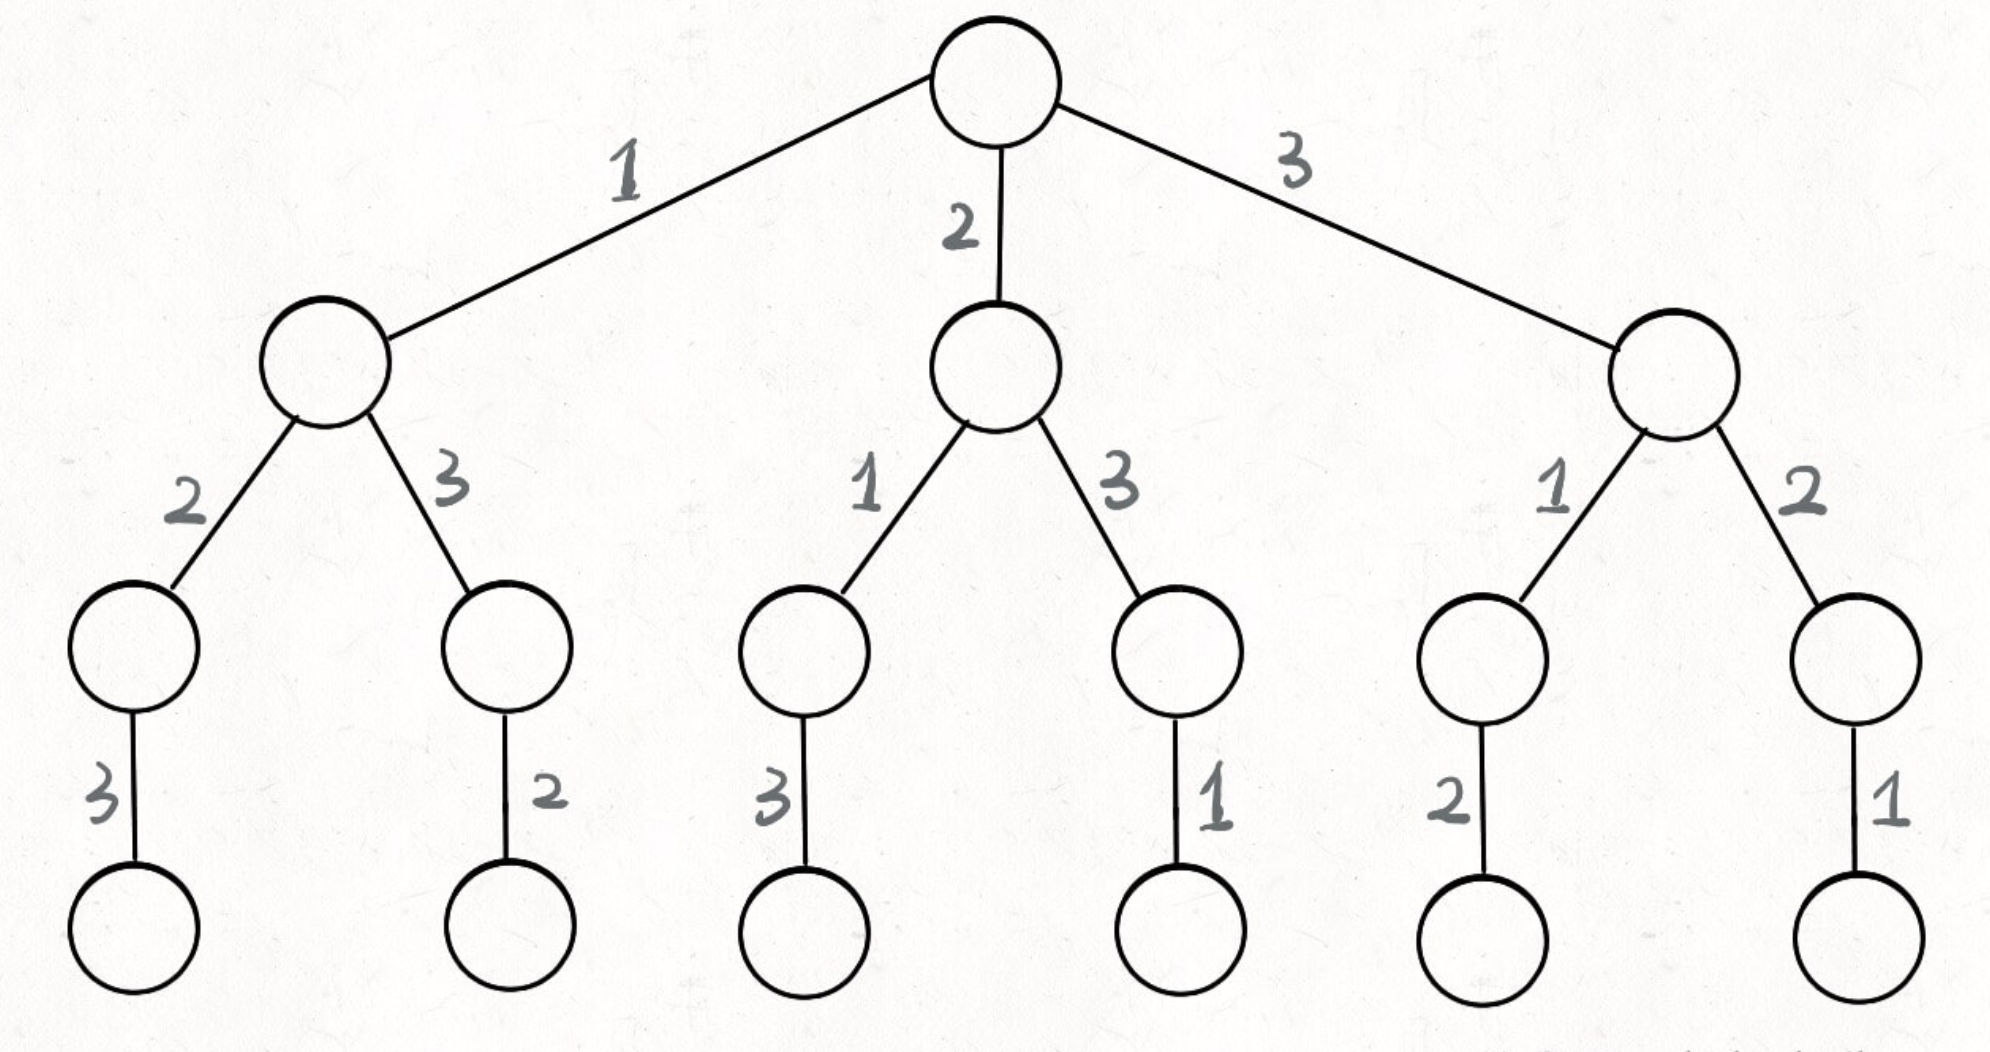
\includegraphics[width=.5\textwidth]{fig/Backtrack_1.png}
\end{figure}

只要从根遍历这棵树,记录路径上的数字,其实就是所有的全排列。我们不妨把这棵树称为回溯算法的「决策树」。

为啥说这是决策树呢,因为你在每个节点上其实都在做决策。比如说你站在下图的红色节点上:
\begin{figure}[H]
    \centering
    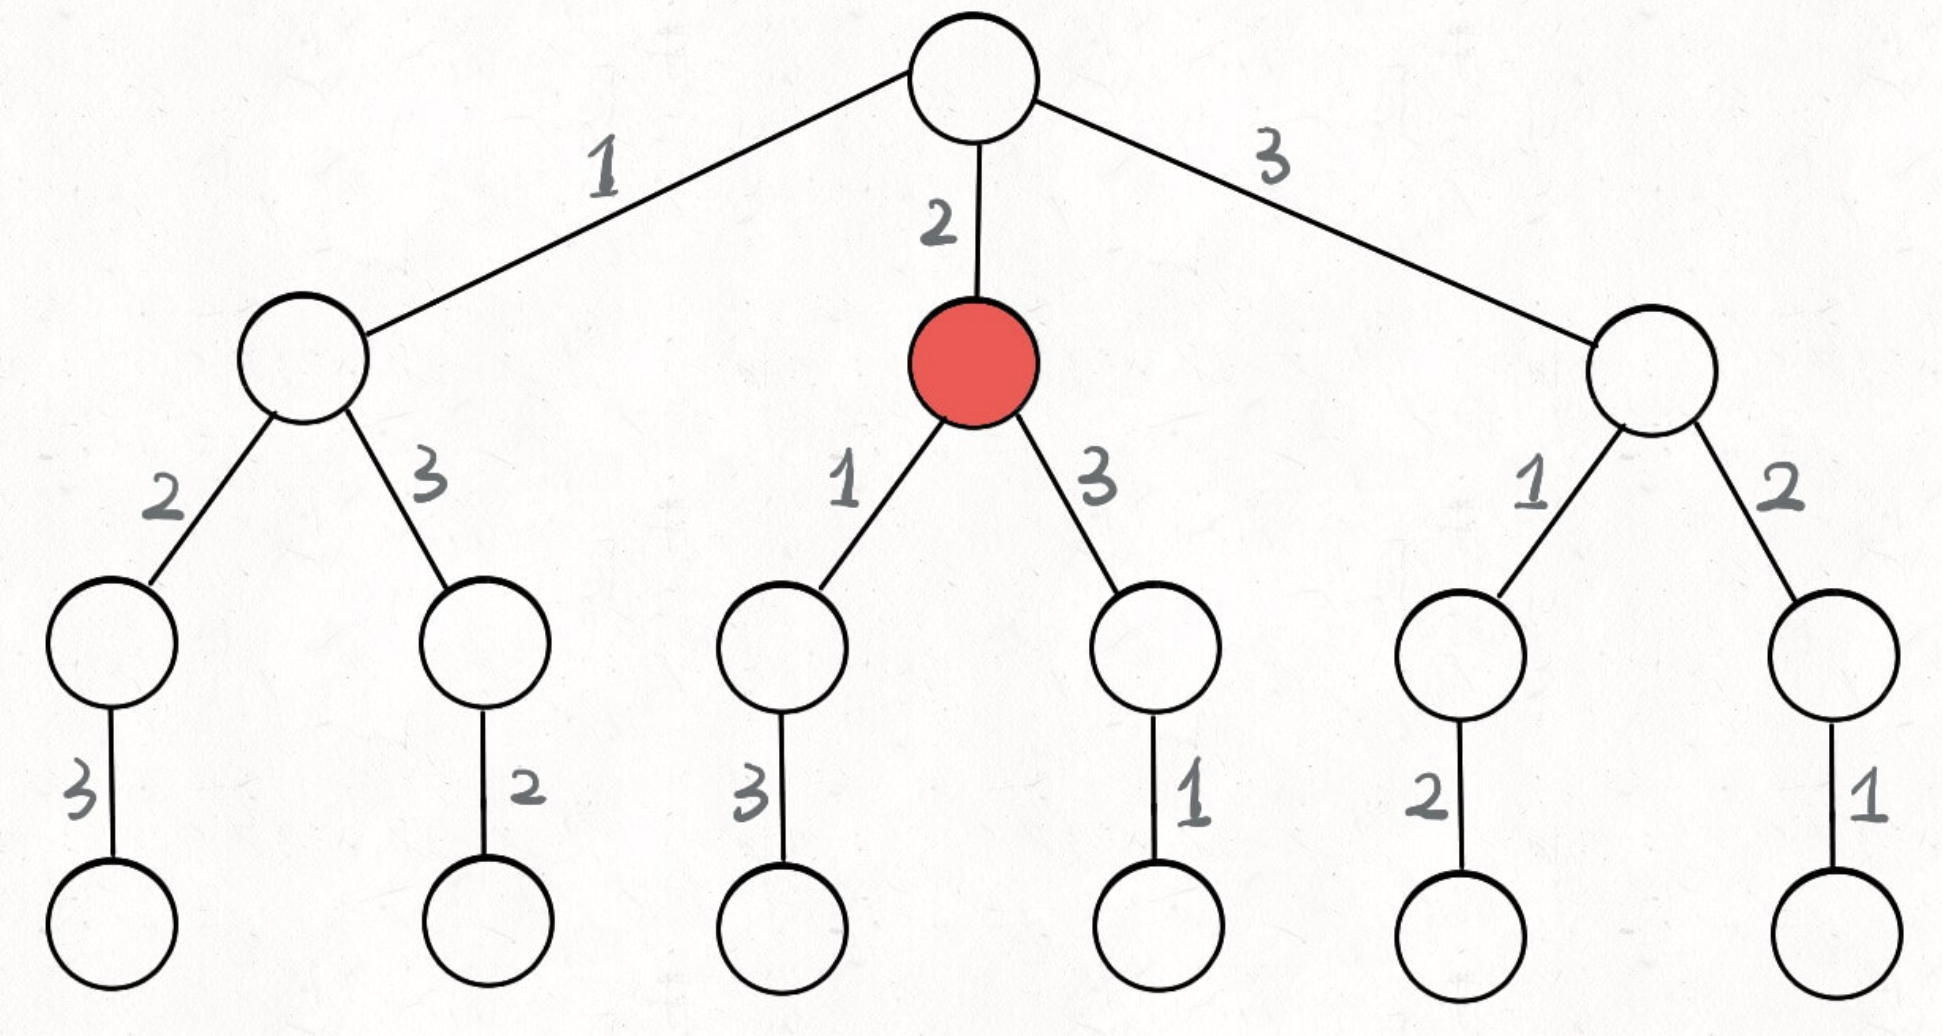
\includegraphics[width=.5\textwidth]{fig/Backtrack_2.png}
\end{figure}

你现在就在做决策,可以选择 1 那条树枝,也可以选择 3 那条树枝。为啥只能在 1 和 3 之中选择呢?因为 2 这个树枝在你身后,这个选择你之前做过了,而全排列是不允许重复使用数字的。

现在可以解答开头的几个名词:[2] 就是「路径」,记录你已经做过的选择;[1,3] 就是「选择列表」,表示你当前可以做出的选择;「结束条件」就是遍历到树的底层,在这里就是选择列表为空的时候。

如果明白了这几个名词,可以把「路径」和「选择」列表作为决策树上每个节点的属性,比如下图列出了几个节点的属性:
\begin{figure}[H]
    \centering
    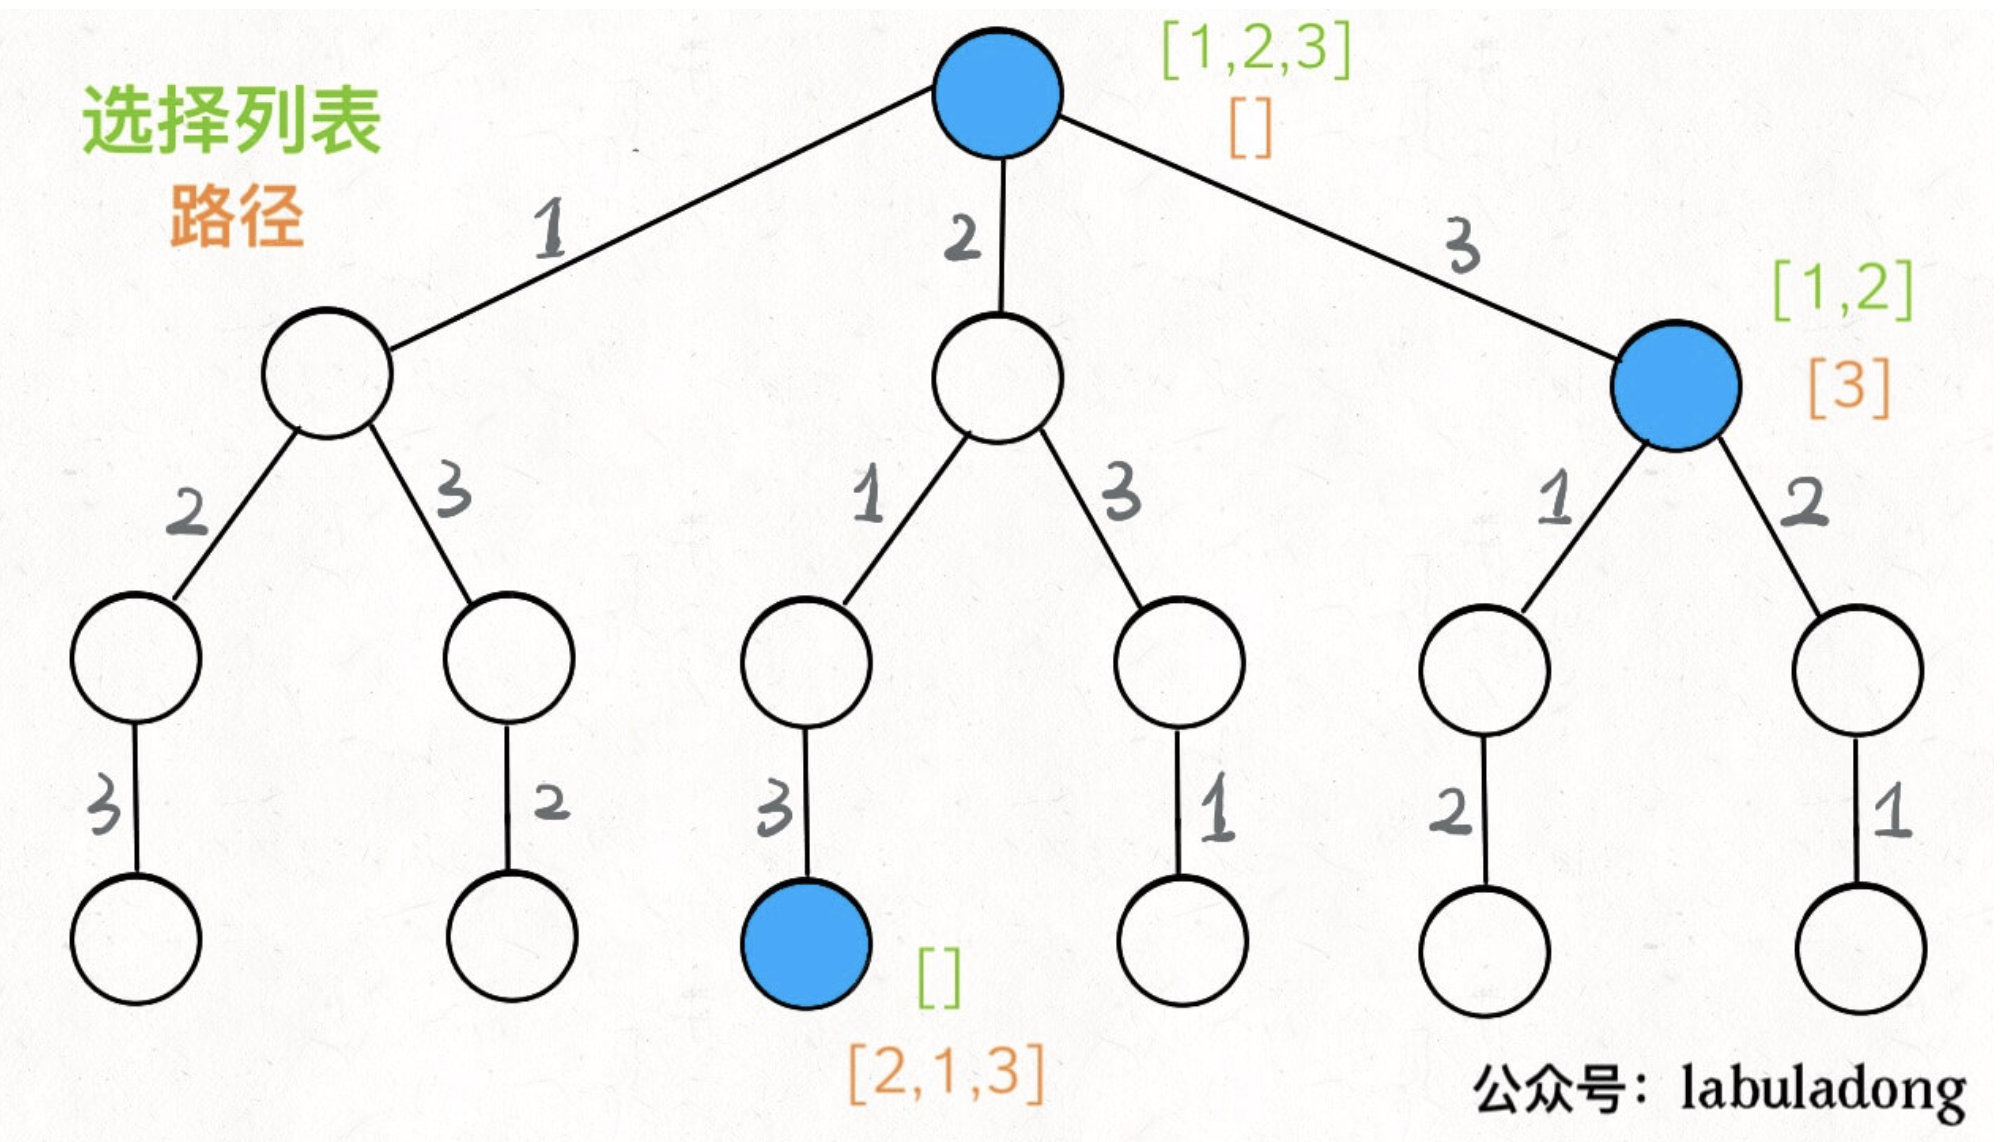
\includegraphics[width=.5\textwidth]{fig/Backtrack_3.png}
\end{figure}

我们定义的 backtrack 函数其实就像一个指针,在这棵树上游走,同时要正确维护每个节点的属性,每当走到树的底层,其「路径」就是一个全排列。

再进一步,如何遍历一棵树?这个应该不难吧。回忆一下之前「学习数据结构的框架思维」写过,各种搜索问题其实都是树的遍历问题,而多叉树的遍历框架就是这样:
\begin{lstlisting}
void traverse(TreeNode root) {
    for (TreeNode child : root.childern)
        // 前序遍历需要的操作
        traverse(child);
        // 后序遍历需要的操作
}
\end{lstlisting}

而所谓的前序遍历和后序遍历,他们只是两个很有用的时间点,我给你画张图你就明白了:
\begin{figure}[H]
    \centering
    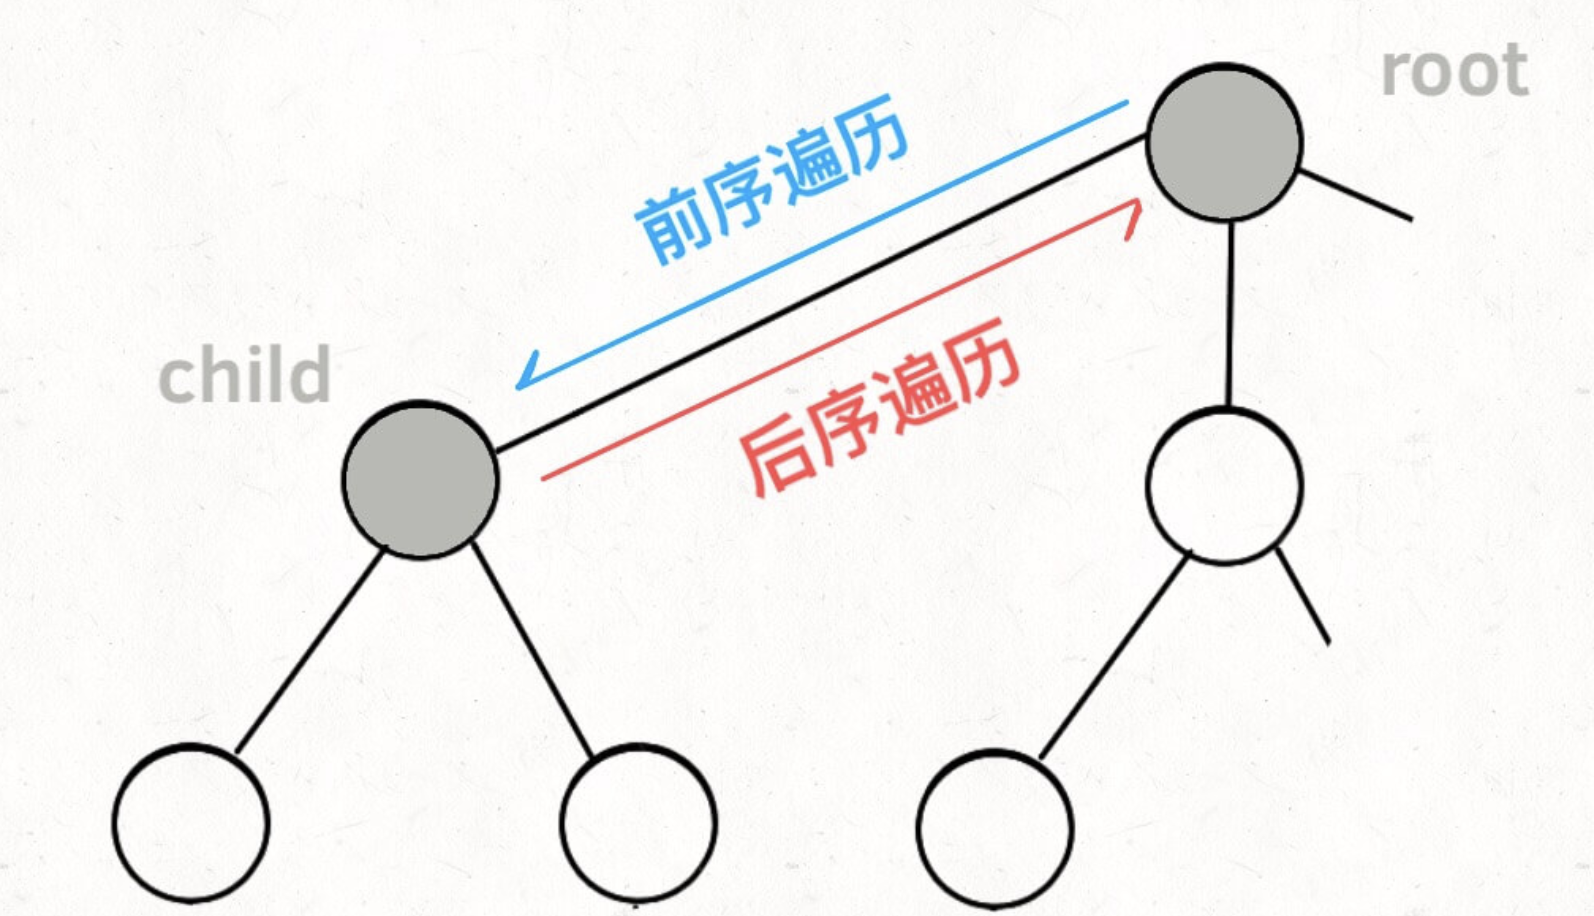
\includegraphics[width=.5\textwidth]{fig/Backtrack_4.png}
\end{figure}

前序遍历的代码在进入某一个节点之前的那个时间点执行,后序遍历代码在离开某个节点之后的那个时间点执行。

回想我们刚才说的,「路径」和「选择」是每个节点的属性,函数在树上游走要正确维护节点的属性,那么就要在这两个特殊时间点搞点动作:
\begin{figure}[H]
    \centering
    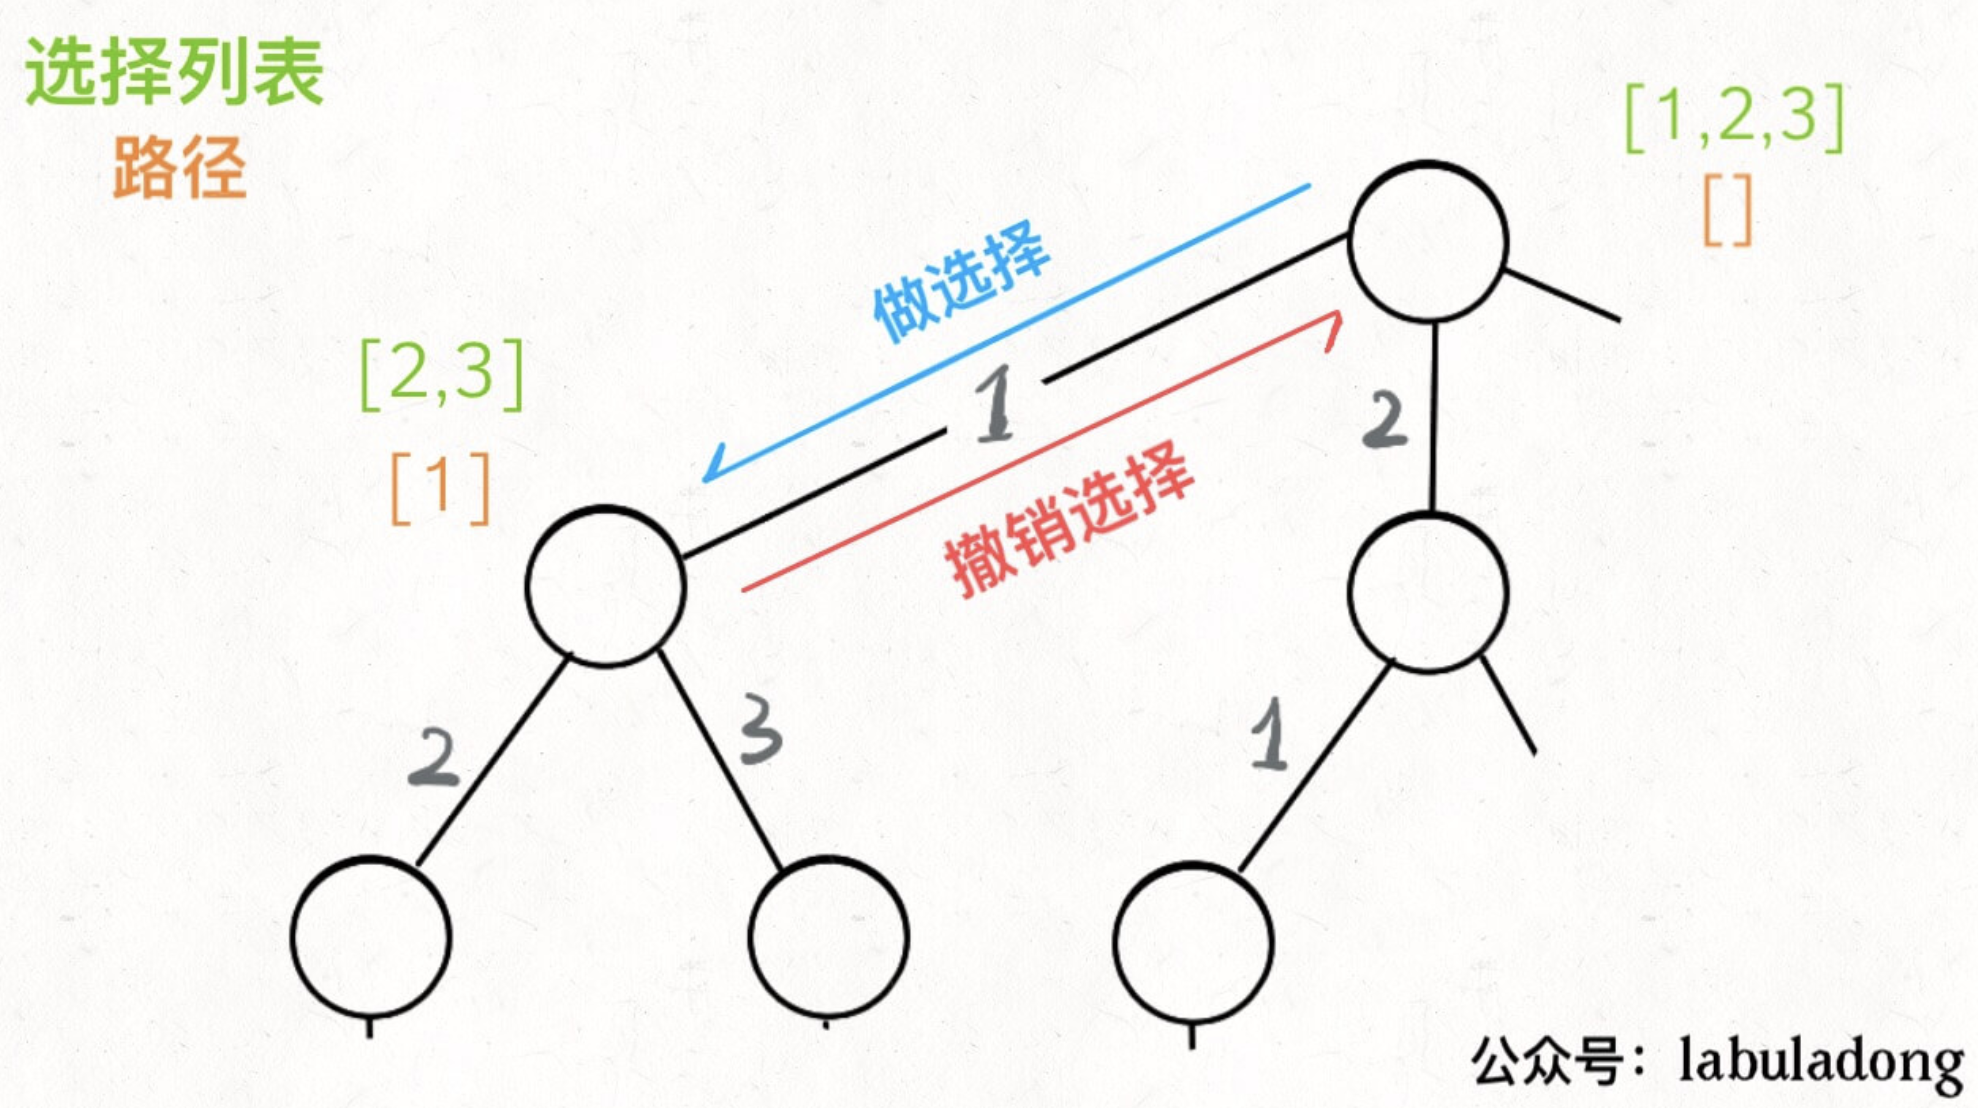
\includegraphics[width=.5\textwidth]{fig/Backtrack_5.png}
\end{figure}

现在,你是否理解了回溯算法的这段核心框架?
\begin{lstlisting}
for 选择 in 选择列表:
    # 做选择
    将该选择从选择列表移除
    路径.add(选择)
    backtrack(路径, 选择列表)
    # 撤销选择
    路径.remove(选择)
    将该选择再加入选择列表
\end{lstlisting}

\textbf{我们只要在递归之前做出选择,在递归之后撤销刚才的选择,就能正确得到每个节点的选择列表和路径}。

\begin{framed}
\textbf{理解:
\begin{itemize}
\setlength{\itemsep}{0pt}
\setlength{\parsep}{0pt}
\setlength{\parskip}{0pt}
    \item 做选择相当于在决策树中向下走一步;
    \item 撤销选择相当于在决策树中回退一步;
\end{itemize}
}
\end{framed}

下面,直接看全排列代码:
\begin{lstlisting}
List<List<Integer>> res = new LinkedList<>();

/* 主函数,输入一组不重复的数字,返回它们的全排列 */
List<List<Integer>> permute(int[] nums) {
    // 记录「路径」
    LinkedList<Integer> track = new LinkedList<>();
    backtrack(nums, track);
    return res;
}

// 路径:记录在 track 中
// 选择列表:nums 中不存在于 track 的那些元素
// 结束条件:nums 中的元素全都在 track 中出现
void backtrack(int[] nums, LinkedList<Integer> track) {
    // 触发结束条件
    if (track.size() == nums.length) {
        res.add(new LinkedList(track));
        return;
    }
    
    for (int i = 0; i < nums.length; i++) {
        // 排除不合法的选择
        if (track.contains(nums[i]))
            continue;
        // 做选择
        track.add(nums[i]);
        // 进入下一层决策树
        backtrack(nums, track);
        // 取消选择
        track.removeLast();
    }
}
\end{lstlisting}

我们这里稍微做了些变通,没有显式记录「选择列表」,而是通过 nums 和 track 推导出当前的选择列表:
\begin{figure}[H]
    \centering
    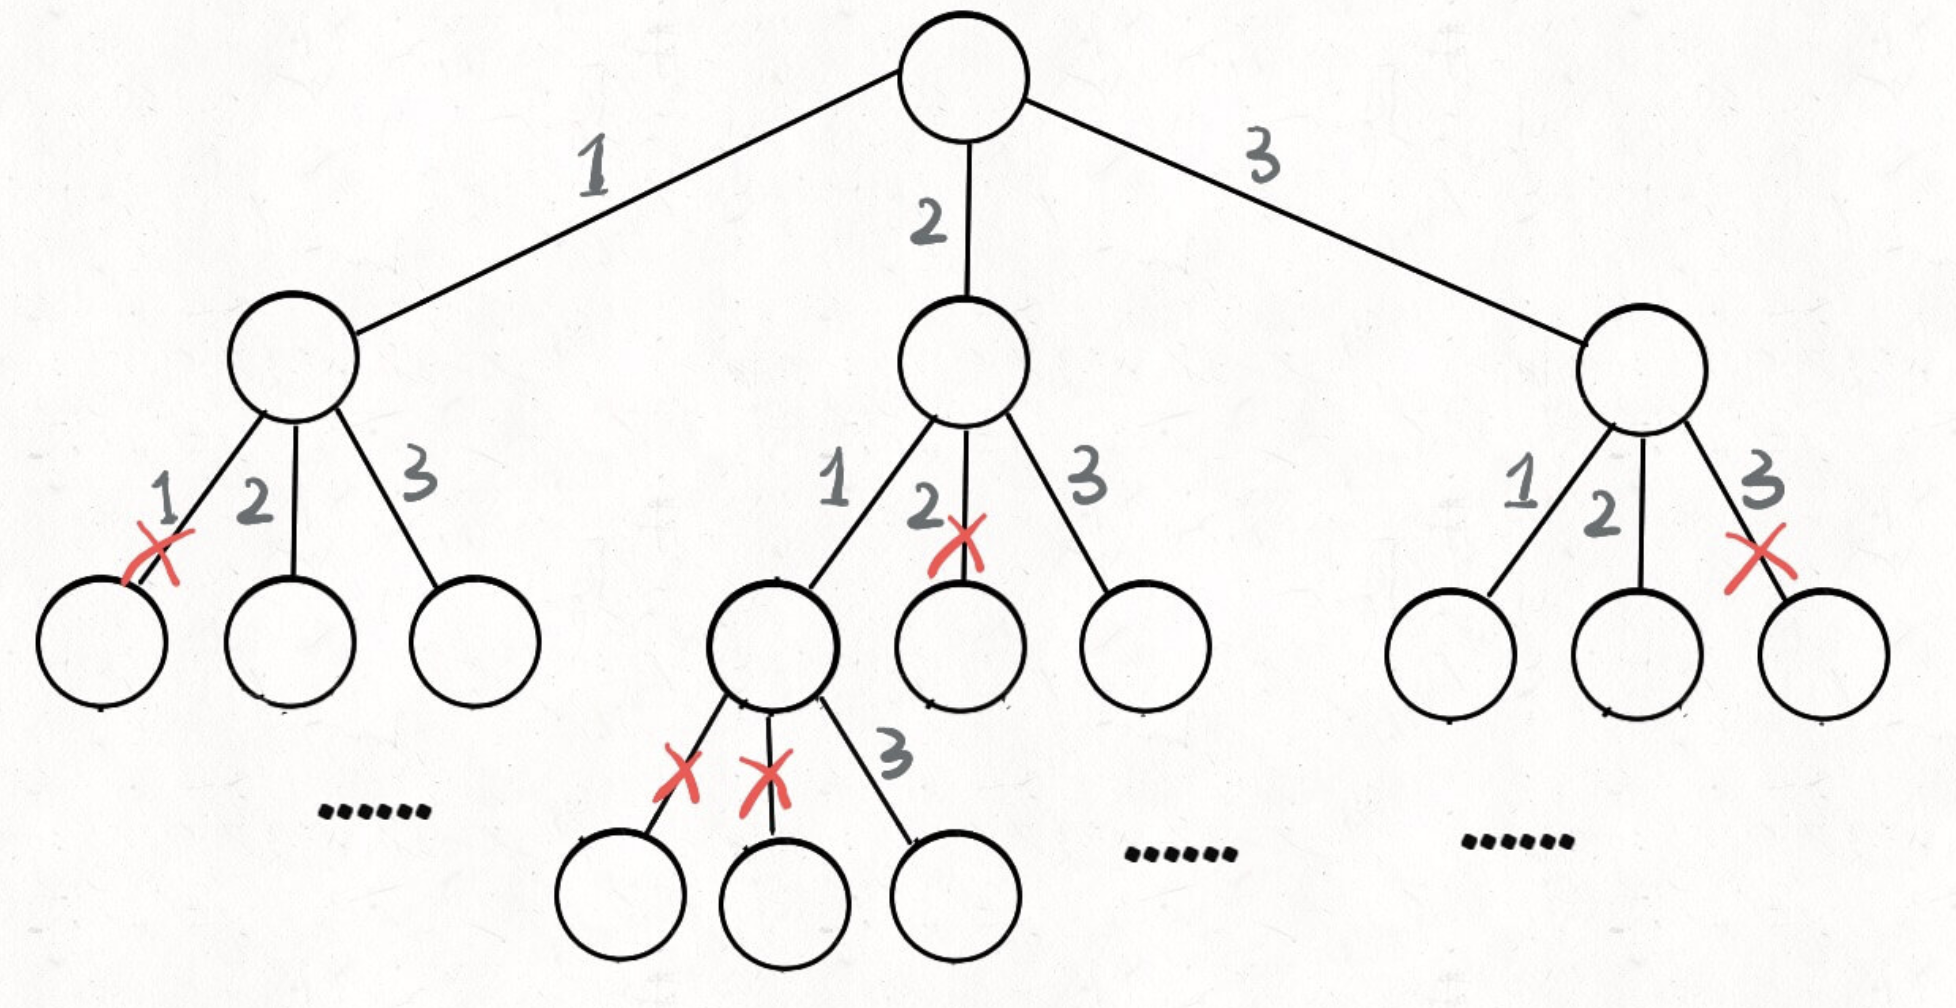
\includegraphics[width=.5\textwidth]{fig/Backtrack_6.png}
\end{figure}

至此,我们就通过全排列问题详解了回溯算法的底层原理。当然,这个算法解决全排列不是很高效,应为对链表使用 contains 方法需要 O(N) 的时间复杂度。有更好的方法通过交换元素达到目的,但是难理解一些,这里就不写了,有兴趣可以自行搜索一下。

但是必须说明的是,不管怎么优化,都符合回溯框架,而且时间复杂度都不可能低于 $O(N!)$,因为穷举整棵决策树是无法避免的。这也是回溯算法的一个特点,不像动态规划存在重叠子问题可以优化,回溯算法就是纯暴力穷举,复杂度一般都很高。

明白了全排列问题,就可以直接套回溯算法框架了,下面简单看看 N 皇后问题。

\subsection{N 皇后问题}
这个问题很经典了,简单解释一下:给你一个 N×N 的棋盘,让你放置 N 个皇后,使得它们不能互相攻击。

PS:皇后可以攻击同一行、同一列、左上左下右上右下四个方向的任意单位。

这个问题本质上跟全排列问题差不多,决策树的每一层表示棋盘上的每一行;每个节点可以做出的选择是,在该行的任意一列放置一个皇后。

直接套用框架:
\begin{lstlisting}
vector<vector<string>> res;

/* 输入棋盘边长 n,返回所有合法的放置 */
vector<vector<string>> solveNQueens(int n) {
    // '.' 表示空,'Q' 表示皇后,初始化空棋盘。
    vector<string> board(n, string(n, '.'));
    backtrack(board, 0);
    return res;
}

// 路径:board 中小于 row 的那些行都已经成功放置了皇后
// 选择列表:第 row 行的所有列都是放置皇后的选择
// 结束条件:row 超过 board 的最后一行
void backtrack(vector<string>& board, int row) {
    // 触发结束条件
    if (row == board.size()) {
        res.push_back(board);
        return;
    }
    
    int n = board[row].size();
    for (int col = 0; col < n; col++) {
        // 排除不合法选择
        if (!isValid(board, row, col)) 
            continue;
        // 做选择
        board[row][col] = 'Q';
        // 进入下一行决策
        backtrack(board, row + 1);
        // 撤销选择
        board[row][col] = '.';
    }
}
\end{lstlisting}

这部分主要代码,其实跟全排列问题差不多,isValid 函数的实现也很简单:
\begin{lstlisting}
/* 是否可以在 board[row][col] 放置皇后? */
bool isValid(vector<string>& board, int row, int col) {
    int n = board.size();
    // 检查列是否有皇后互相冲突
    for (int i = 0; i < n; i++) {
        if (board[i][col] == 'Q')
            return false;
    }
    // 检查右上方是否有皇后互相冲突
    for (int i = row - 1, j = col + 1; 
            i >= 0 && j < n; i--, j++) {
        if (board[i][j] == 'Q')
            return false;
    }
    // 检查左上方是否有皇后互相冲突
    for (int i = row - 1, j = col - 1;
            i >= 0 && j >= 0; i--, j--) {
        if (board[i][j] == 'Q')
            return false;
    }
    return true;
}
\end{lstlisting}

函数 backtrack 依然像个在决策树上游走的指针,通过 row 和 col 就可以表示函数遍历到的位置,通过 isValid 函数可以将不符合条件的情况剪枝:
\begin{figure}[H]
    \centering
    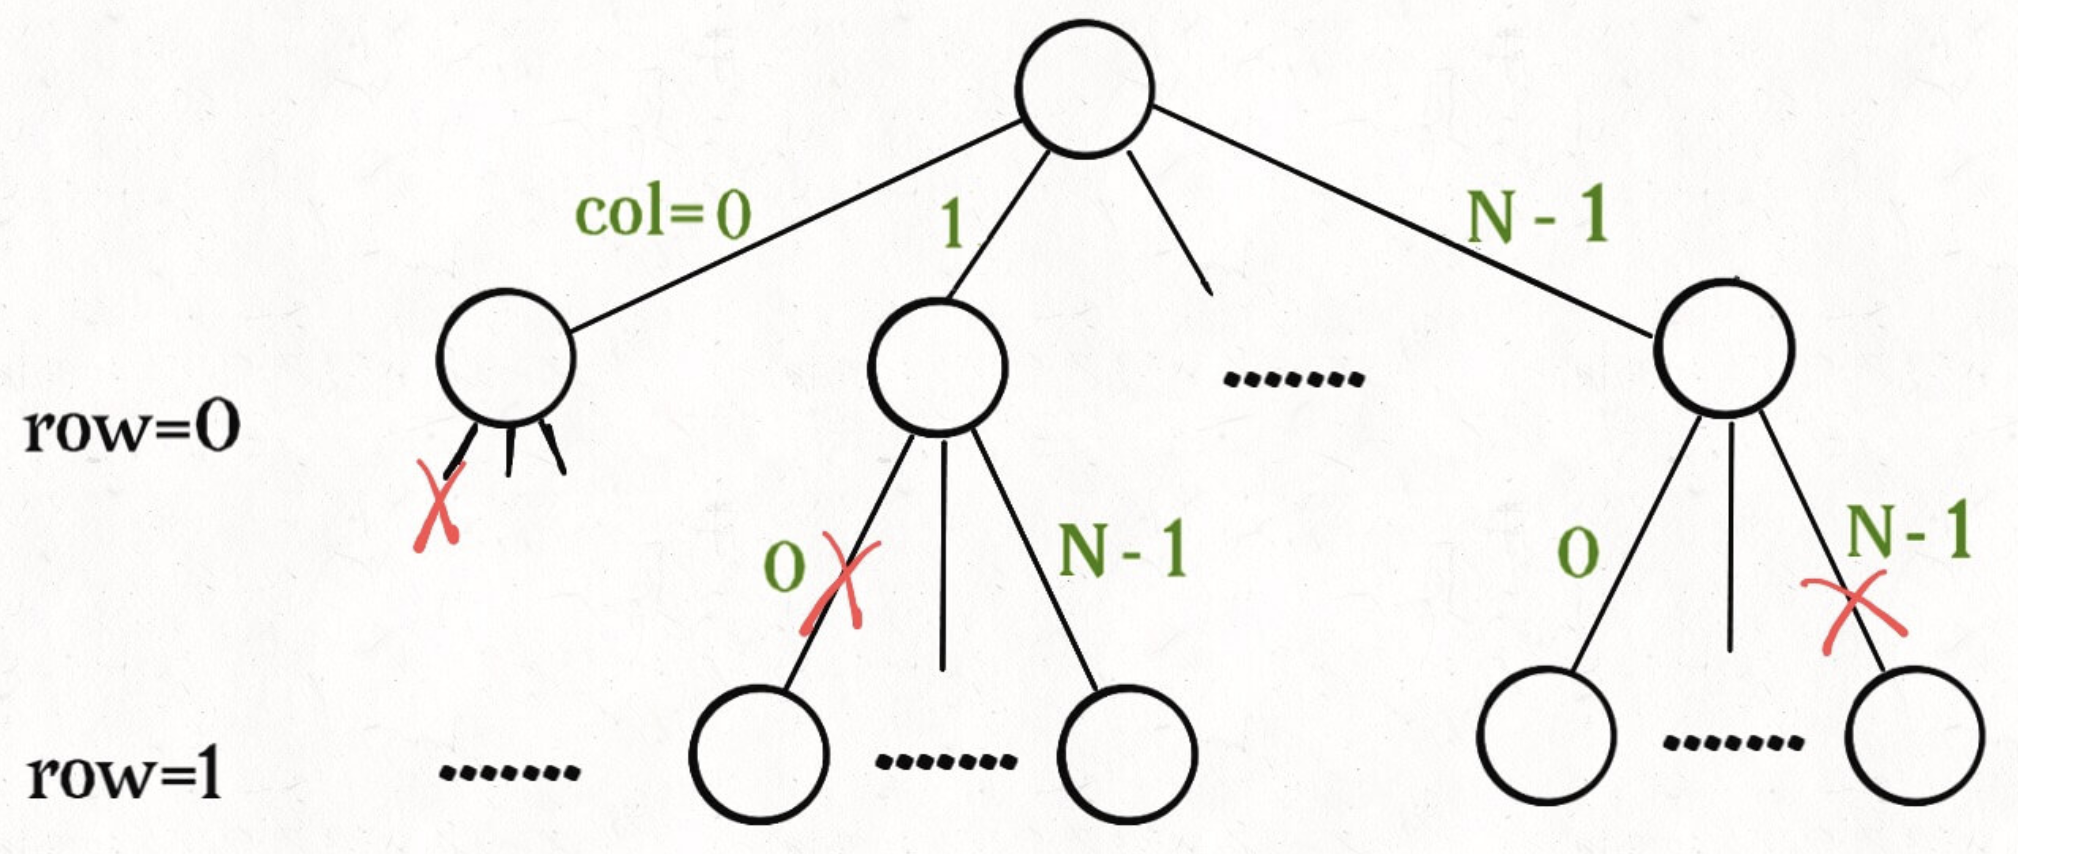
\includegraphics[width=.5\textwidth]{fig/Backtrack_7.png}
\end{figure}

如果直接给你这么一大段解法代码,可能是懵逼的。但是现在明白了回溯算法的框架套路,还有啥难理解的呢?无非是改改做选择的方式,排除不合法选择的方式而已,只要框架存于心,你面对的只剩下小问题了。

当 N = 8 时,就是八皇后问题,数学大佬高斯穷尽一生都没有数清楚八皇后问题到底有几种可能的放置方法,但是我们的算法只需要一秒就可以算出来所有可能的结果。不过真的不怪高斯。这个问题的复杂度确实非常高,看看我们的决策树,虽然有 isValid 函数剪枝,但是最坏时间复杂度仍然是 $O(N^(N+1))$,而且无法优化。如果 N = 10 的时候,计算就已经很耗时了。

有的时候,我们并不想得到所有合法的答案,只想要一个答案,怎么办呢?比如解数独的算法,找所有解法复杂度太高,只要找到一种解法就可以。

其实特别简单,只要稍微修改一下回溯算法的代码即可:
\begin{lstlisting}
// 函数找到一个答案后就返回 true
bool backtrack(vector<string>& board, int row) {
    // 触发结束条件
    if (row == board.size()) {
        res.push_back(board);
        return true;
    }
    ...
    for (int col = 0; col < n; col++) {
        ...
        board[row][col] = 'Q';

        if (backtrack(board, row + 1))
            return true;
        
        board[row][col] = '.';
    }

    return false;
}
\end{lstlisting}

这样修改后,只要找到一个答案,for 循环的后续递归穷举都会被阻断。也许你可以在 N 皇后问题的代码框架上,稍加修改,写一个解数独的算法?

\subsection{最后总结}
回溯算法就是个多叉树的遍历问题,关键就是在前序遍历和后序遍历的位置做一些操作,算法框架如下:
\begin{lstlisting}
def backtrack(...):
    for 选择 in 选择列表:
        做选择
        backtrack(...)
        撤销选择
\end{lstlisting}

写 backtrack 函数时,需要维护走过的「路径」和当前可以做的「选择列表」,当触发「结束条件」时,将「路径」记入结果集。

其实想想看,回溯算法和动态规划是不是有点像呢?我们在动态规划系列文章中多次强调,动态规划的三个需要明确的点就是「状态」「选择」和「base case」,是不是就对应着走过的「路径」,当前的「选择列表」和「结束条件」?

某种程度上说,动态规划的暴力求解阶段就是回溯算法。只是有的问题具有重叠子问题性质,可以用 dp table 或者备忘录优化,将递归树大幅剪枝,这就变成了动态规划。而今天的两个问题,都没有重叠子问题,也就是回溯算法问题了,复杂度非常高是不可避免的。

\section{子集排列组合}
\url{https://github.com/labuladong/fucking-algorithm/blob/master/%E9%AB%98%E9%A2%91%E9%9D%A2%E8%AF%95%E7%B3%BB%E5%88%97/%E5%AD%90%E9%9B%86%E6%8E%92%E5%88%97%E7%BB%84%E5%90%88.md}

今天就来聊三道考察频率高,而且容易让人搞混的算法问题,分别是求子集(subset),求排列(permutation),求组合(combination)。

这几个问题都可以用回溯算法模板解决,同时子集问题还可以用数学归纳思想解决。读者可以记住这几个问题的回溯套路,就不怕搞不清了。

\subsection{子集}
问题很简单,输入一个不包含重复数字的数组,要求算法输出这些数字的所有子集。
\begin{lstlisting}
vector<vector<int>> subsets(vector<int>& nums);
\end{lstlisting}

比如输入 nums = [1,2,3],你的算法应输出 8 个子集,包含空集和本身,顺序可以不同:
\begin{lstlisting}
[ [],[1],[2],[3],[1,3],[2,3],[1,2],[1,2,3] ]
\end{lstlisting}

\subsubsection{利用数学归纳的思想}
假设我现在知道了规模更小的子问题的结果,如何推导出当前问题的结果呢?

具体来说就是,现在让你求 [1,2,3] 的子集,如果你知道了 [1,2] 的子集,是否可以推导出 [1,2,3] 的子集呢?先把 [1,2] 的子集写出来瞅瞅:
\begin{lstlisting}
[ [],[1],[2],[1,2] ]
\end{lstlisting}

你会发现这样一个规律:
\begin{lstlisting}
subset([1,2,3]) - subset([1,2]) = = [3],[1,3],[2,3],[1,2,3]
\end{lstlisting}

而这个结果,就是把 sebset([1,2]) 的结果中每个集合再添加上 3。

换句话说,如果 A = subset([1,2]) ,那么:subset([1,2,3]) = A + [A[i].add(3) for i = 1..len(A)]

这就是一个典型的递归结构嘛,[1,2,3] 的子集可以由 [1,2] 追加得出,[1,2] 的子集可以由 [1] 追加得出,base case 显然就是当输入集合为空集时,输出子集也就是一个空集。

翻译成代码就很容易理解了:
\begin{lstlisting}
vector<vector<int>> subsets(vector<int>& nums) {
    // base case,返回一个空集
    if (nums.empty()) return {{}};
    // 把最后一个元素拿出来
    int n = nums.back();
    nums.pop_back();
    // 先递归算出前面元素的所有子集
    vector<vector<int>> res = subsets(nums);

    int size = res.size();
    for (int i = 0; i < size; i++) {
        // 然后在之前的结果之上追加
        res.push_back(res[i]);
        res.back().push_back(n);
    }
    return res;
}
\end{lstlisting}

这个问题的时间复杂度计算比较容易坑人。我们之前说的计算递归算法时间复杂度的方法,是找到递归深度,然后乘以每次递归中迭代的次数。对于这个问题,递归深度显然是 N,但我们发现每次递归 for 循环的迭代次数取决于 res 的长度,并不是固定的。

根据刚才的思路,res 的长度应该是每次递归都翻倍,所以说总的迭代次数应该是 $2^N$。或者不用这么麻烦,你想想一个大小为 N 的集合的子集总共有几个?$2^N$ 个对吧,所以说至少要对 res 添加 $2^N$ 次元素。

那么算法的时间复杂度就是 $O(2^N)$ 吗?还是不对,$2^N$ 个子集是 push\_back 添加进 res 的,所以要考虑 push
\_back 这个操作的效率:
\begin{lstlisting}
for (int i = 0; i < size; i++) {
    res.push_back(res[i]); // O(N)
    res.back().push_back(n); // O(1)
}
\end{lstlisting}

因为 res[i] 也是一个数组呀,push\_back 是把 res[i] copy 一份然后添加到数组的最后,所以一次操作的时间是 O(N)。

综上,总的时间复杂度就是 $O(N*2^N)$,还是比较耗时的。

空间复杂度的话,如果不计算储存返回结果所用的空间的,只需要 O(N) 的递归堆栈空间。如果计算 res 所需的空间,应该是 $O(N*2^N)$。

\subsubsection{通用方法——回溯算法}
回溯算法的模板:
\begin{lstlisting}
result = []
def backtrack(路径, 选择列表):
    if 满足结束条件:
        result.add(路径)
        return
    for 选择 in 选择列表:
        做选择
        backtrack(路径, 选择列表)
        撤销选择
\end{lstlisting}

只要改造回溯算法的模板就行了:
\begin{lstlisting}
vector<vector<int>> res;

vector<vector<int>> subsets(vector<int>& nums) {
    // 记录走过的路径
    vector<int> track;
    backtrack(nums, 0, track);
    return res;
}

void backtrack(vector<int>& nums, int start, vector<int>& track) {
    res.push_back(track);
    for (int i = start; i < nums.size(); i++) {
        // 做选择
        track.push_back(nums[i]);
        // 回溯
        backtrack(nums, i + 1, track);
        // 撤销选择
        track.pop_back();
    }
}
\end{lstlisting}

可以看见,对 res 更新的位置处在前序遍历,也就是说,res 就是树上的所有节点:
\begin{figure}[H]
    \centering
    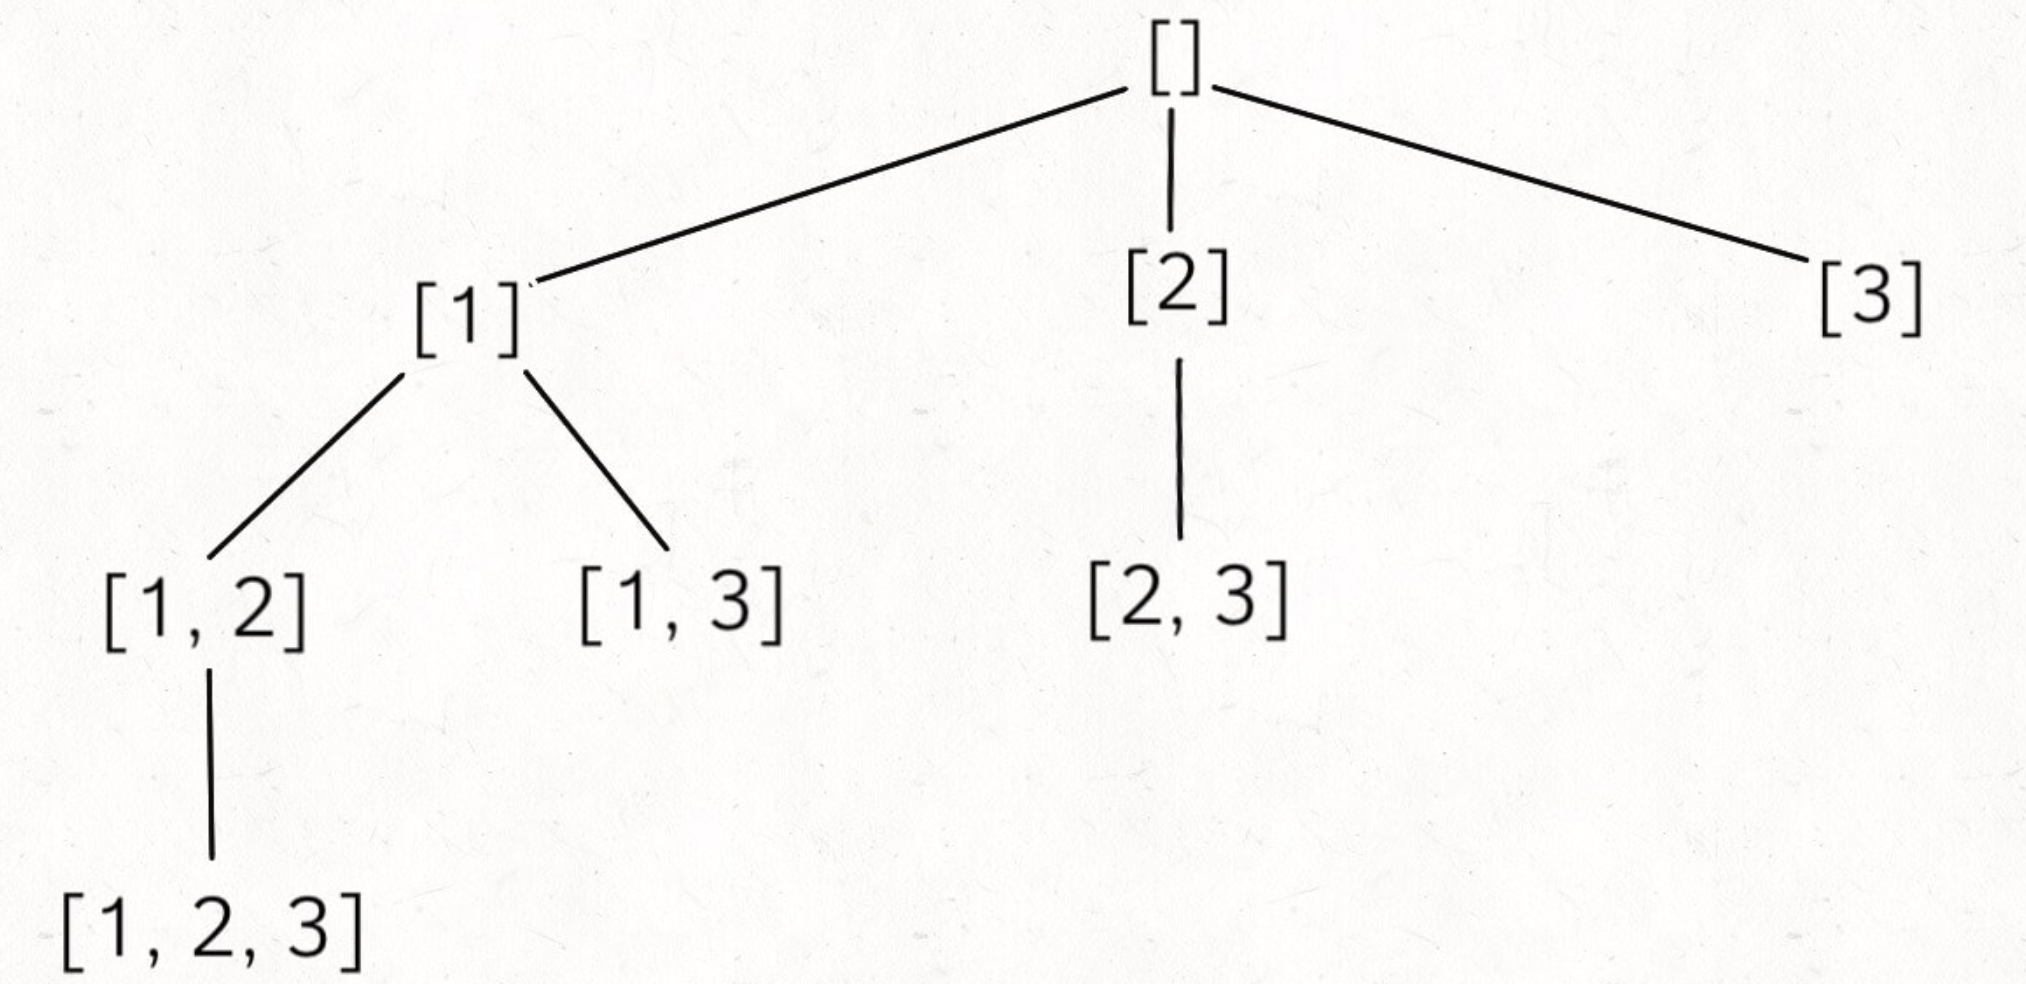
\includegraphics[width=.6\textwidth]{fig/Subset.png}
\end{figure}

\subsection{组合}
输入两个数字 n, k,算法输出 [1..n] 中 k 个数字的所有组合。
\begin{lstlisting}
vector<vector<int>> combine(int n, int k);
\end{lstlisting}

比如输入 n = 4, k = 2,输出如下结果,顺序无所谓,但是不能包含重复(按照组合的定义,[1,2] 和 [2,1] 也算重复):
\begin{lstlisting}
[ [1,2], [1,3], [1,4], [2,3], [2,4], [3,4] ]
\end{lstlisting}

这也是典型的回溯算法,k 限制了树的高度,n 限制了树的宽度,继续套我们以前讲过的回溯算法模板框架就行了:
\begin{figure}[H]
    \centering
    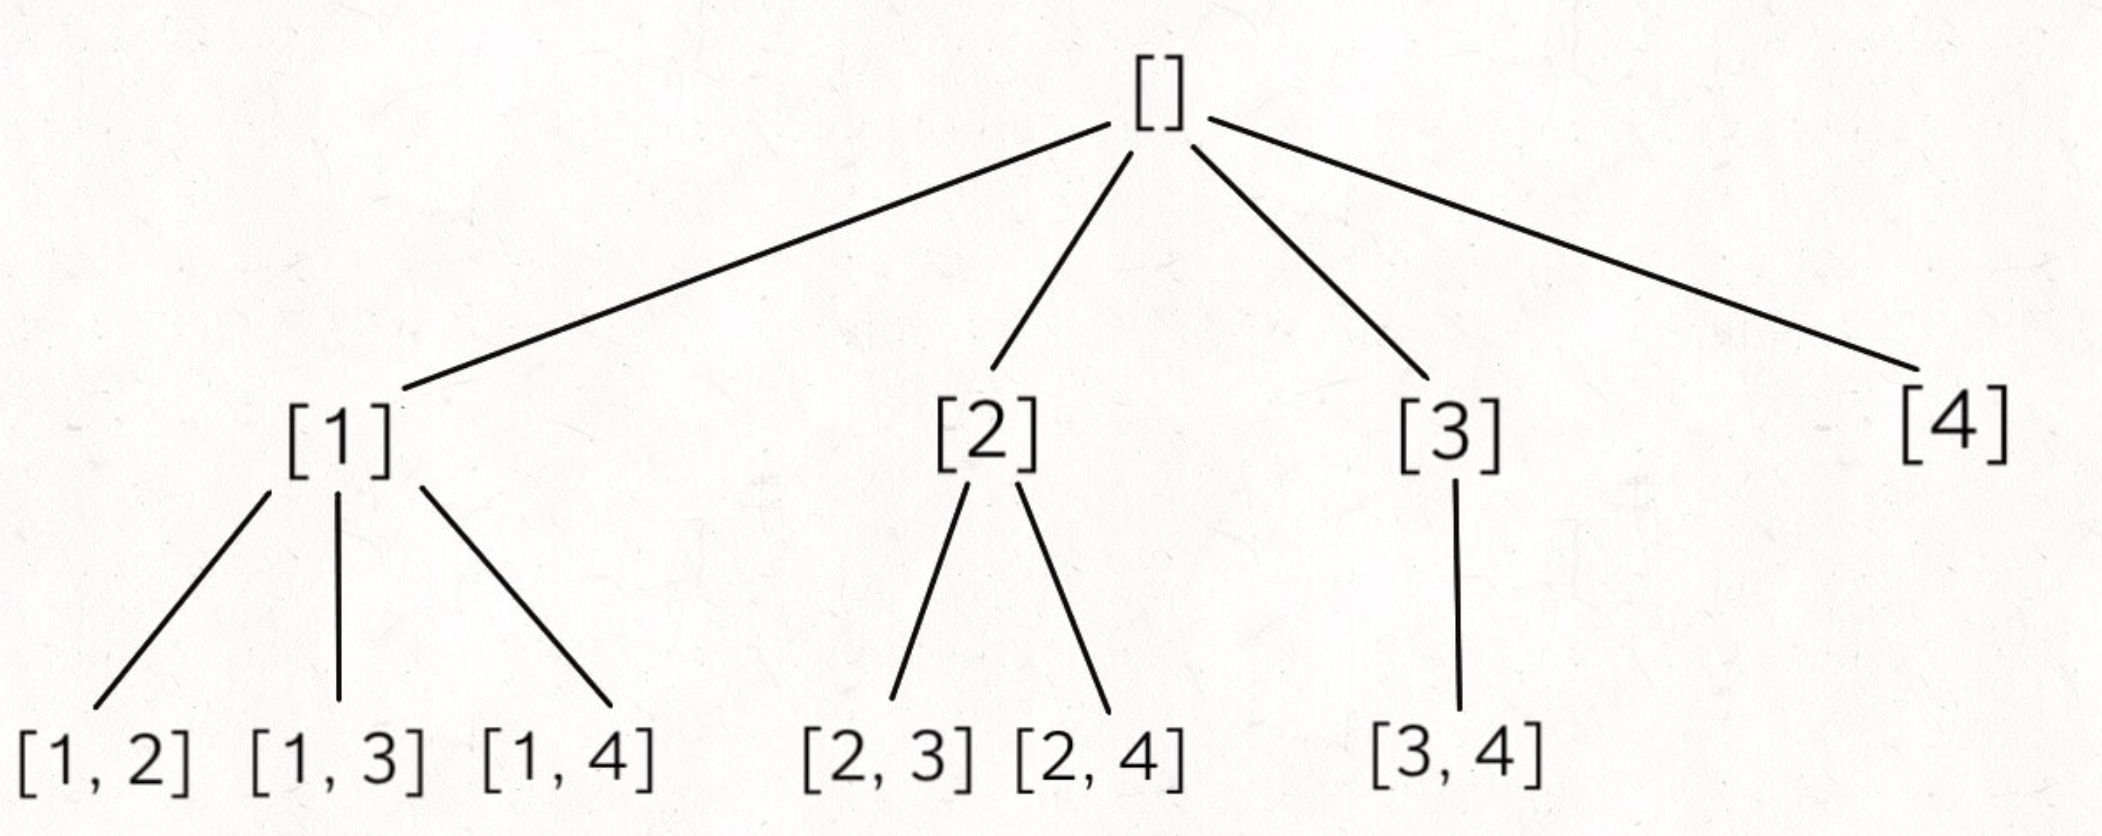
\includegraphics[width=.6\textwidth]{fig/Combination.png}
\end{figure}

\begin{lstlisting}
vector<vector<int>>res;

vector<vector<int>> combine(int n, int k) {
    if (k <= 0 || n <= 0) return res;
    vector<int> track;
    backtrack(n, k, 1, track);
    return res;
}

void backtrack(int n, int k, int start, vector<int>& track) {
    // 到达树的底部
    if (k == track.size()) {
        res.push_back(track);
        return;
    }
    // 注意 i 从 start 开始递增
    for (int i = start; i <= n; i++) {
        // 做选择
        track.push_back(i);
        backtrack(n, k, i + 1, track);
        // 撤销选择
        track.pop_back();
    }
}
\end{lstlisting}

backtrack 函数和计算子集的差不多,区别在于,更新 res 的时机是树到达底端时。

\subsection{排列}
输入一个不包含重复数字的数组 nums,返回这些数字的全部排列。
\begin{lstlisting}
vector<vector<int>> permute(vector<int>& nums);
\end{lstlisting}

比如说输入数组 [1,2,3],输出结果应该如下,顺序无所谓,不能有重复:
\begin{lstlisting}
[ [1,2,3], [1,3,2], [2,1,3], [2,3,1], [3,1,2], [3,2,1] ]
\end{lstlisting}

「回溯算法详解」中就是拿这个问题来解释回溯模板的。这里又列出这个问题,是将「排列」和「组合」这两个回溯算法的代码拿出来对比。

首先画出回溯树来看一看:
\begin{figure}[H]
    \centering
    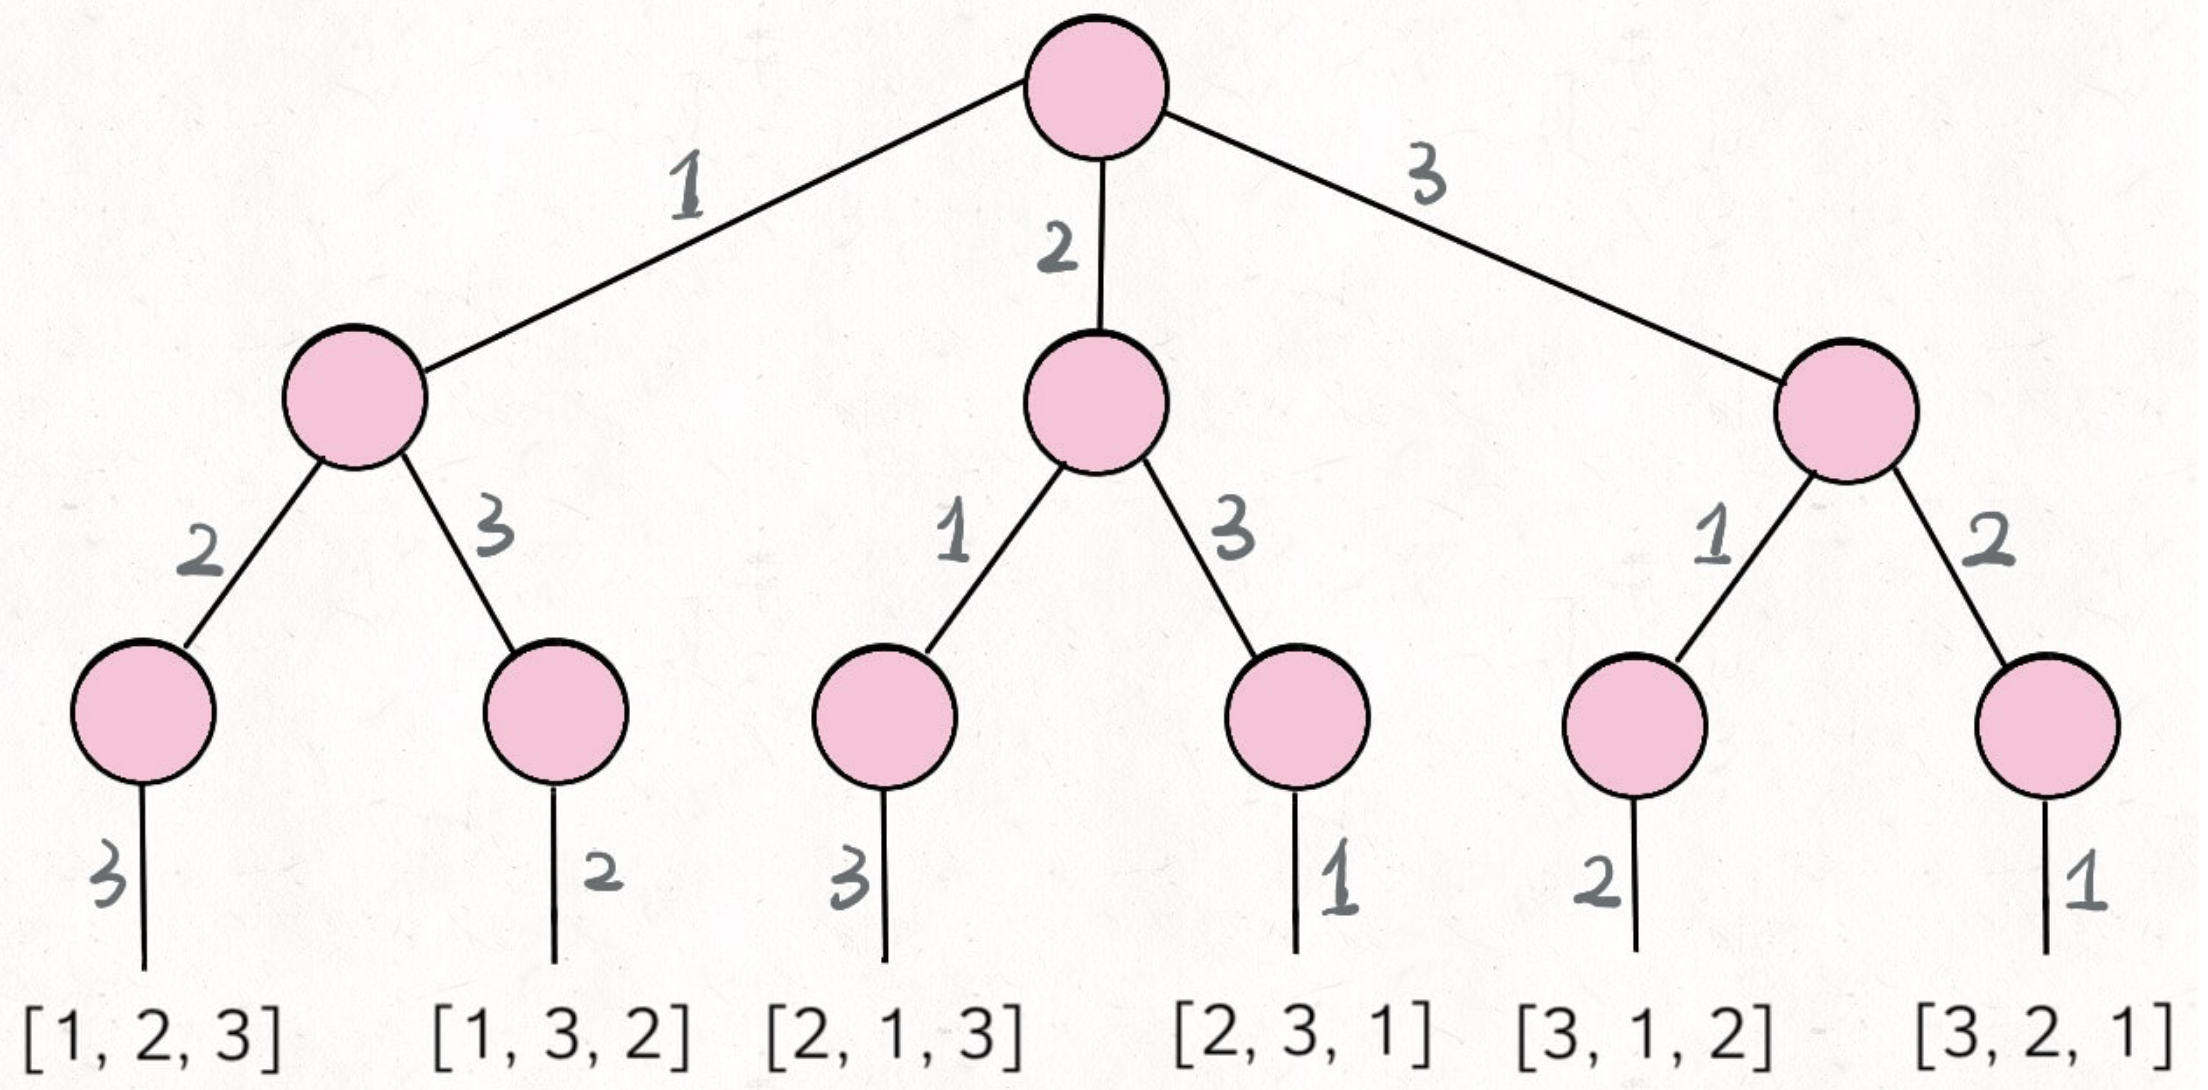
\includegraphics[width=.6\textwidth]{fig/Permutation.png}
\end{figure}

C++解法代码:
\begin{lstlisting}
class Solution {
public:
    vector<vector<int>> permute(vector<int>& nums) {
        paths.clear();
        path.clear();

        vector<int> used(nums.size(),false);

        helper(nums,used);

        return paths;
    }
private:
    void helper(vector<int>& nums,vector<int>& used) {
        if(path.size() == nums.size()) {
            paths.push_back(path);
            return ;
        }

        for(int i = 0 ; i < nums.size() ; ++i) {
            if(used[i]) continue;

            used[i] = true;
            path.push_back(nums[i]);
            
            helper(nums,used);

            path.pop_back();
            used[i] = false;
        }
    }
private:
    vector<vector<int>> paths;
    vector<int> path;
};
\end{lstlisting}

回溯模板依然没有变,但是根据排列问题和组合问题画出的树来看,排列问题的树比较对称,而组合问题的树越靠右节点越少。

在代码中的体现就是,排列问题每次通过 contains 方法来排除在 track 中已经选择过的数字;而组合问题通过传入一个 start 参数,来排除 start 索引之前的数字。

\subsection{总结}
子集问题可以利用数学归纳思想,假设已知一个规模较小的问题的结果,思考如何推导出原问题的结果。也可以用回溯算法,要用 start 参数排除已选择的数字。

组合问题利用的是回溯思想,结果可以表示成树结构,我们只要套用回溯算法模板即可,关键点在于要用一个 start 排除已经选择过的数字。

排列问题是回溯思想,也可以表示成树结构套用算法模板,关键点在于使用 contains 方法排除已经选择的数字,前文有详细分析,这里主要是和组合问题作对比。

\section{二分查找}
\url{https://github.com/labuladong/fucking-algorithm/blob/master/%E7%AE%97%E6%B3%95%E6%80%9D%E7%BB%B4%E7%B3%BB%E5%88%97/%E4%BA%8C%E5%88%86%E6%9F%A5%E6%89%BE%E8%AF%A6%E8%A7%A3.md}

先给大家讲个笑话乐呵一下:

有一天阿东到图书馆借了 N 本书,出图书馆的时候,警报响了,于是保安把阿东拦下,要检查一下哪本书没有登记出借。阿东正准备把每一本书在报警器下过一下,以找出引发警报的书,但是保安露出不屑的眼神:你连二分查找都不会吗?于是保安把书分成两堆,让第一堆过一下报警器,报警器响;于是再把这堆书分成两堆…… 最终,检测了 logN 次之后,保安成功的找到了那本引起警报的书,露出了得意和嘲讽的笑容。于是阿东背着剩下的书走了。

从此,图书馆丢了 N - 1 本书。

二分查找并不简单,Knuth 大佬(发明 KMP 算法的那位)都说二分查找:\textbf{思路很简单,细节是魔鬼}。很多人喜欢拿整型溢出的 bug 说事儿,但是二分查找真正的坑根本就不是那个细节问题,而是在于到底要给 mid 加一还是减一,while 里到底用 <= 还是 <。

本文就来探究几个最常用的二分查找场景:寻找一个数、寻找左侧边界、寻找右侧边界。而且,我们就是要深入细节,比如不等号是否应该带等号,mid 是否应该加一等等。分析这些细节的差异以及出现这些差异的原因,保证你能灵活准确地写出正确的二分查找算法。

\subsection{二分查找框架}
\begin{lstlisting}
int binarySearch(int[] nums, int target) {
    int left = 0, right = ...;

    while(...) {
        int mid = left + (right - left) / 2;
        if (nums[mid] == target) {
            ...
        } else if (nums[mid] < target) {
            left = ...
        } else if (nums[mid] > target) {
            right = ...
        }
    }
    return ...;
}
\end{lstlisting}

分析二分查找的一个技巧是:\textbf{不要出现 else,而是把所有情况用 else if 写清楚,这样可以清楚地展现所有细节}。本文都会使用 else if,旨在讲清楚,读者理解后可自行简化。

其中 ... 标记的部分,就是可能出现细节问题的地方,当你见到一个二分查找的代码时,首先注意这几个地方。后文用实例分析这些地方能有什么样的变化。

另外声明一下,\textbf{计算 mid 时需要防止溢出},代码中 left + (right - left) / 2 就和 (left + right) / 2 的结果相同,但是有效防止了 left 和 right 太大直接相加导致溢出。

\subsection{寻找一个数(基本的二分搜索)}
这个场景是最简单的,可能也是大家最熟悉的,即搜索一个数,如果存在,返回其索引,否则返回 -1。
\begin{lstlisting}
int binarySearch(int[] nums, int target) {
    int left = 0; 
    int right = nums.length - 1; // 注意

    while(left <= right) {
        int mid = left + (right - left) / 2;
        if(nums[mid] == target)
            return mid; 
        else if (nums[mid] < target)
            left = mid + 1; // 注意
        else if (nums[mid] > target)
            right = mid - 1; // 注意
    }
    return -1;
}
\end{lstlisting}

\subsubsection{为什么 while 循环的条件中是 <=,而不是 <?}
答:因为初始化 right 的赋值是 nums.length - 1,即最后一个元素的索引,而不是 nums.length。

这二者可能出现在不同功能的二分查找中,区别是:前者相当于两端都闭区间 [left, right],后者相当于左闭右开区间 [left, right),因为索引大小为 nums.length 是越界的。

我们这个算法中使用的是前者 [left, right] 两端都闭的区间。\textbf{这个区间其实就是每次进行搜索的区间}。

什么时候应该停止搜索呢?当然,找到了目标值的时候可以终止:
\begin{lstlisting}
if(nums[mid] == target)
        return mid; 
\end{lstlisting}

但如果没找到,就需要 while 循环终止,然后返回 -1。那 while 循环什么时候应该终止?搜索区间为空的时候应该终止,意味着你没得找了,就等于没找到嘛。

while(left <= right) 的终止条件是 left == right + 1,写成区间的形式就是 [right + 1, right],或者带个具体的数字进去 [3, 2],可见这时候区间为空,因为没有数字既大于等于 3 又小于等于 2 的吧。所以这时候 while 循环终止是正确的,直接返回 -1 即可。

while(left < right) 的终止条件是 left == right,写成区间的形式就是 [left, right],或者带个具体的数字进去 [2, 2],这时候区间非空,还有一个数 2,但此时 while 循环终止了。也就是说这区间 [2, 2] 被漏掉了,索引 2 没有被搜索,如果这时候直接返回 -1 就是错误的。

当然,如果你非要用 while(left < right) 也可以,我们已经知道了出错的原因,就打个补丁好了:
\begin{lstlisting}
 //...
    while(left < right) {
        // ...
    }
    return nums[left] == target ? left : -1;
\end{lstlisting}

\subsubsection{为什么 left = mid + 1,right = mid - 1?}
我看有的代码是 right = mid 或者 left = mid,没有这些加加减减,到底怎么回事,怎么判断?

答:这也是二分查找的一个难点,不过只要你能理解前面的内容,就能够很容易判断。

刚才明确了「搜索区间」这个概念,而且本算法的搜索区间是两端都闭的,即 [left, right]。那么当我们发现索引 mid 不是要找的 target 时,下一步应该去搜索哪里呢?

当然是去搜索 [left, mid-1] 或者 [mid+1, right] 对不对?因为 mid 已经搜索过,应该从搜索区间中去除。

\subsubsection{此算法有什么缺陷?}
答:至此,你应该已经掌握了该算法的所有细节,以及这样处理的原因。但是,这个算法存在局限性。

比如说给你有序数组 nums = [1,2,2,2,3],target 为 2,此算法返回的索引是 2,没错。但是如果我想得到 target 的左侧边界,即索引 1,或者我想得到 target 的右侧边界,即索引 3,这样的话此算法是无法处理的。

这样的需求很常见,你也许会说,找到一个 target,然后向左或向右线性搜索不行吗?可以,但是不好,因为这样难以保证二分查找对数级的复杂度了。

我们后续的算法就来讨论这两种二分查找的算法。

\subsection{寻找左侧边界的二分搜索}
以下是最常见的代码形式,其中的标记是需要注意的细节:
\begin{lstlisting}
int left_bound(int[] nums, int target) {
    if (nums.length == 0) return -1;
    int left = 0;
    int right = nums.length; // 注意
    
    while (left < right) { // 注意
        int mid = (left + right) / 2;
        if (nums[mid] == target) {
            right = mid;
        } else if (nums[mid] < target) {
            left = mid + 1;
        } else if (nums[mid] > target) {
            right = mid; // 注意
        }
    }
    return left;
}
\end{lstlisting}

\subsubsection{为什么 while 中是 < 而不是 <=?}
答:用相同的方法分析,因为 right = nums.length 而不是 nums.length - 1。因此每次循环的「搜索区间」是 [left, right) 左闭右开。

while(left < right) 终止的条件是 left == right,此时搜索区间 [left, left) 为空,所以可以正确终止。

PS:这里先要说一个搜索左右边界和上面这个算法的一个区别,也是很多读者问的:刚才的 right 不是 nums.length - 1 吗,为啥这里非要写成 nums.length 使得「搜索区间」变成左闭右开呢?

因为对于搜索左右侧边界的二分查找,这种写法比较普遍,我就拿这种写法举例了,保证你以后遇到这类代码可以理解。你非要用两端都闭的写法反而更简单,我会在后面写相关的代码,把三种二分搜索都用一种两端都闭的写法统一起来,你耐心往后看就行了。

\subsubsection{为什么没有返回 -1 的操作?如果 nums 中不存在 target 这个值,怎么办?}

答:因为要一步一步来,先理解一下这个「左侧边界」有什么特殊含义:
\begin{figure}[H]
    \centering
    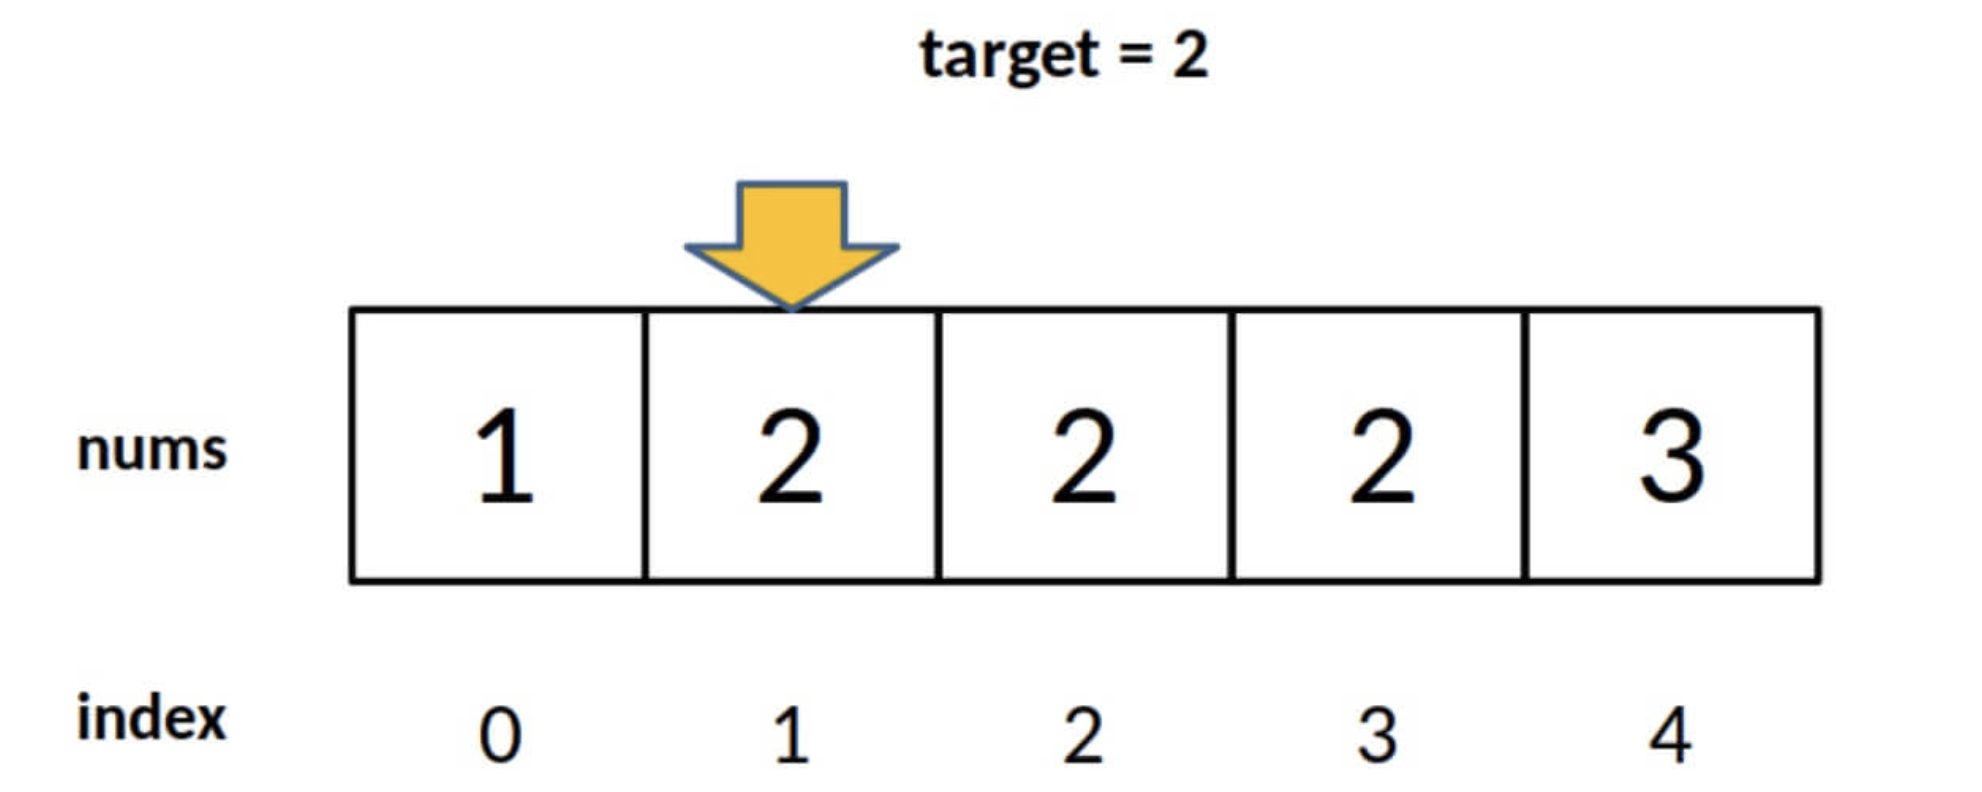
\includegraphics[width=1\textwidth]{fig/Binary_Search_1.png}
\end{figure}

对于这个数组,算法会返回 1。这个 1 的含义可以这样解读:nums 中小于 2 的元素有 1 个。

比如对于有序数组 nums = [2,3,5,7], target = 1,算法会返回 0,含义是:nums 中小于 1 的元素有 0 个。

再比如说 nums = [2,3,5,7], target = 8,算法会返回 4,含义是:nums 中小于 8 的元素有 4 个。

综上可以看出,函数的返回值(即 left 变量的值)取值区间是闭区间 [0, nums.length],所以我们简单添加两行代码就能在正确的时候 return -1:
\begin{lstlisting}
while (left < right) {
    //...
}
// target 比所有数都大
if (left == nums.length) return -1;
// 类似之前算法的处理方式
return nums[left] == target ? left : -1;
\end{lstlisting}

\subsubsection{为什么 left = mid + 1,right = mid ?和之前的算法不一样?}
答:这个很好解释,因为我们的「搜索区间」是 [left, right) 左闭右开,所以当 nums[mid] 被检测之后,下一步的搜索区间应该去掉 mid 分割成两个区间,即 [left, mid) 或 [mid + 1, right)。

\subsubsection{为什么该算法能够搜索左侧边界?}
答:关键在于对于 nums[mid] == target 这种情况的处理:
\begin{lstlisting}
if (nums[mid] == target)
        right = mid;
\end{lstlisting}

可见,找到 target 时不要立即返回,而是缩小「搜索区间」的上界 right,在区间 [left, mid) 中继续搜索,即不断向左收缩,达到锁定左侧边界的目的。

\subsubsection{为什么返回 left 而不是 right?}
答:都是一样的,因为 while 终止的条件是 left == right。

\subsubsection{能不能想办法把 right 变成 nums.length - 1}
也就是继续使用两边都闭的「搜索区间」?这样就可以和第一种二分搜索在某种程度上统一起来了。

答:当然可以,只要你明白了「搜索区间」这个概念,就能有效避免漏掉元素,随便你怎么改都行。下面我们严格根据逻辑来修改:

因为你非要让搜索区间两端都闭,所以 right 应该初始化为 nums.length - 1,while 的终止条件应该是 left == right + 1,也就是其中应该用 <=:
\begin{lstlisting}
int left_bound(int[] nums, int target) {
    // 搜索区间为 [left, right]
    int left = 0, right = nums.length - 1;
    while (left <= right) {
        int mid = left + (right - left) / 2;
        // if else ...
    }
\end{lstlisting}

因为搜索区间是两端都闭的,且现在是搜索左侧边界,所以 left 和 right 的更新逻辑如下:
\begin{lstlisting}
if (nums[mid] < target) {
    // 搜索区间变为 [mid+1, right]
    left = mid + 1;
} else if (nums[mid] > target) {
    // 搜索区间变为 [left, mid-1]
    right = mid - 1;
} else if (nums[mid] == target) {
    // 收缩右侧边界
    right = mid - 1;
}
\end{lstlisting}

由于 while 的退出条件是 left == right + 1,所以当 target 比 nums 中所有元素都大时,会存在以下情况使得索引越界:
\begin{figure}[H]
    \centering
    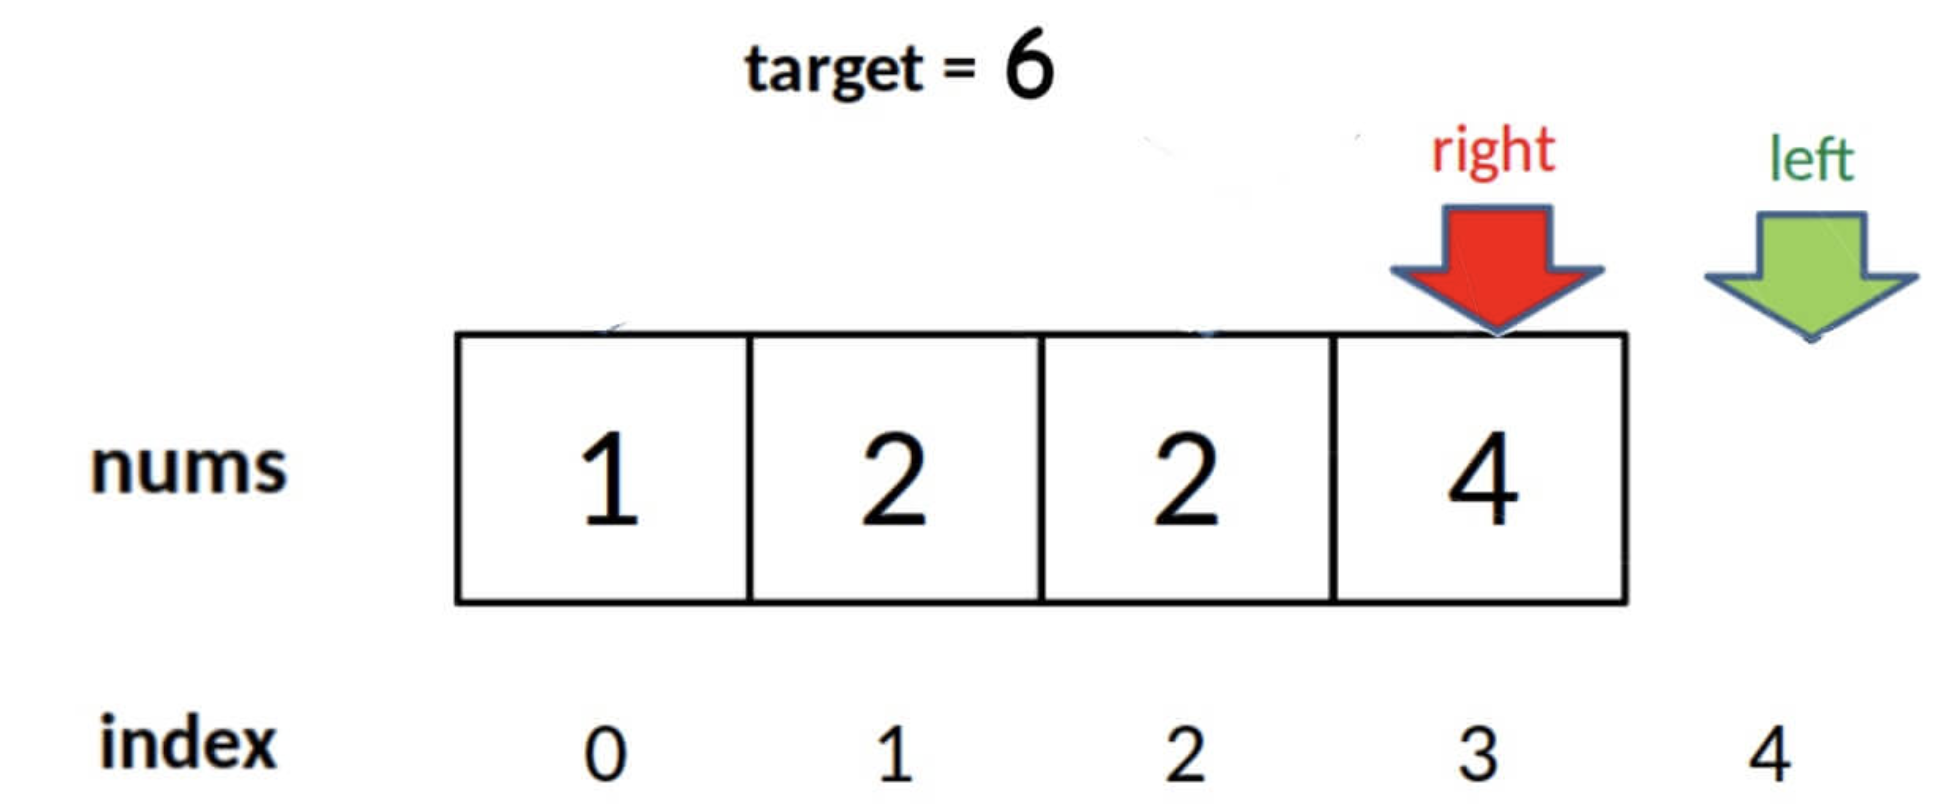
\includegraphics[width=1\textwidth]{fig/Binary_Search_2.png}
\end{figure}

因此,最后返回结果的代码应该检查越界情况:
\begin{lstlisting}
if (left >= nums.length || nums[left] != target)
    return -1;
return left;
\end{lstlisting}

至此,整个算法就写完了,完整代码如下:
\begin{lstlisting}
int left_bound(int[] nums, int target) {
    int left = 0, right = nums.length - 1;
    // 搜索区间为 [left, right]
    while (left <= right) {
        int mid = left + (right - left) / 2;
        if (nums[mid] < target) {
            // 搜索区间变为 [mid+1, right]
            left = mid + 1;
        } else if (nums[mid] > target) {
            // 搜索区间变为 [left, mid-1]
            right = mid - 1;
        } else if (nums[mid] == target) {
            // 收缩右侧边界
            right = mid - 1;
        }
    }
    // 检查出界情况
    if (left >= nums.length || nums[left] != target)
        return -1;
    return left;
}
\end{lstlisting}

\subsection{寻找右侧边界的二分查找}
类似寻找左侧边界的算法,这里也会提供两种写法,还是先写常见的左闭右开的写法,只有两处和搜索左侧边界不同,已标注:
\begin{lstlisting}
int right_bound(int[] nums, int target) {
    if (nums.length == 0) return -1;
    int left = 0, right = nums.length;
    
    while (left < right) {
        int mid = (left + right) / 2;
        if (nums[mid] == target) {
            left = mid + 1; // 注意
        } else if (nums[mid] < target) {
            left = mid + 1;
        } else if (nums[mid] > target) {
            right = mid;
        }
    }
    return left - 1; // 注意
}
\end{lstlisting}

\subsubsection{为什么这个算法能够找到右侧边界?}
答:类似地,关键点还是这里:
\begin{lstlisting}
if (nums[mid] == target) {
    left = mid + 1;
\end{lstlisting}

当 nums[mid] == target 时,不要立即返回,而是增大「搜索区间」的下界 left,使得区间不断向右收缩,达到锁定右侧边界的目的。

\subsubsection{为什么最后返回 left - 1}
为什么最后返回 left - 1 而不像左侧边界的函数,返回 left?而且我觉得这里既然是搜索右侧边界,应该返回 right 才对。

答:首先,while 循环的终止条件是 left == right,所以 left 和 right 是一样的,你非要体现右侧的特点,返回 right - 1 好了。

至于为什么要减一,这是搜索右侧边界的一个特殊点,关键在这个条件判断:
\begin{lstlisting}
if (nums[mid] == target) {
    left = mid + 1;
    // 这样想: mid = left - 1
\end{lstlisting}
\begin{figure}[H]
    \centering
    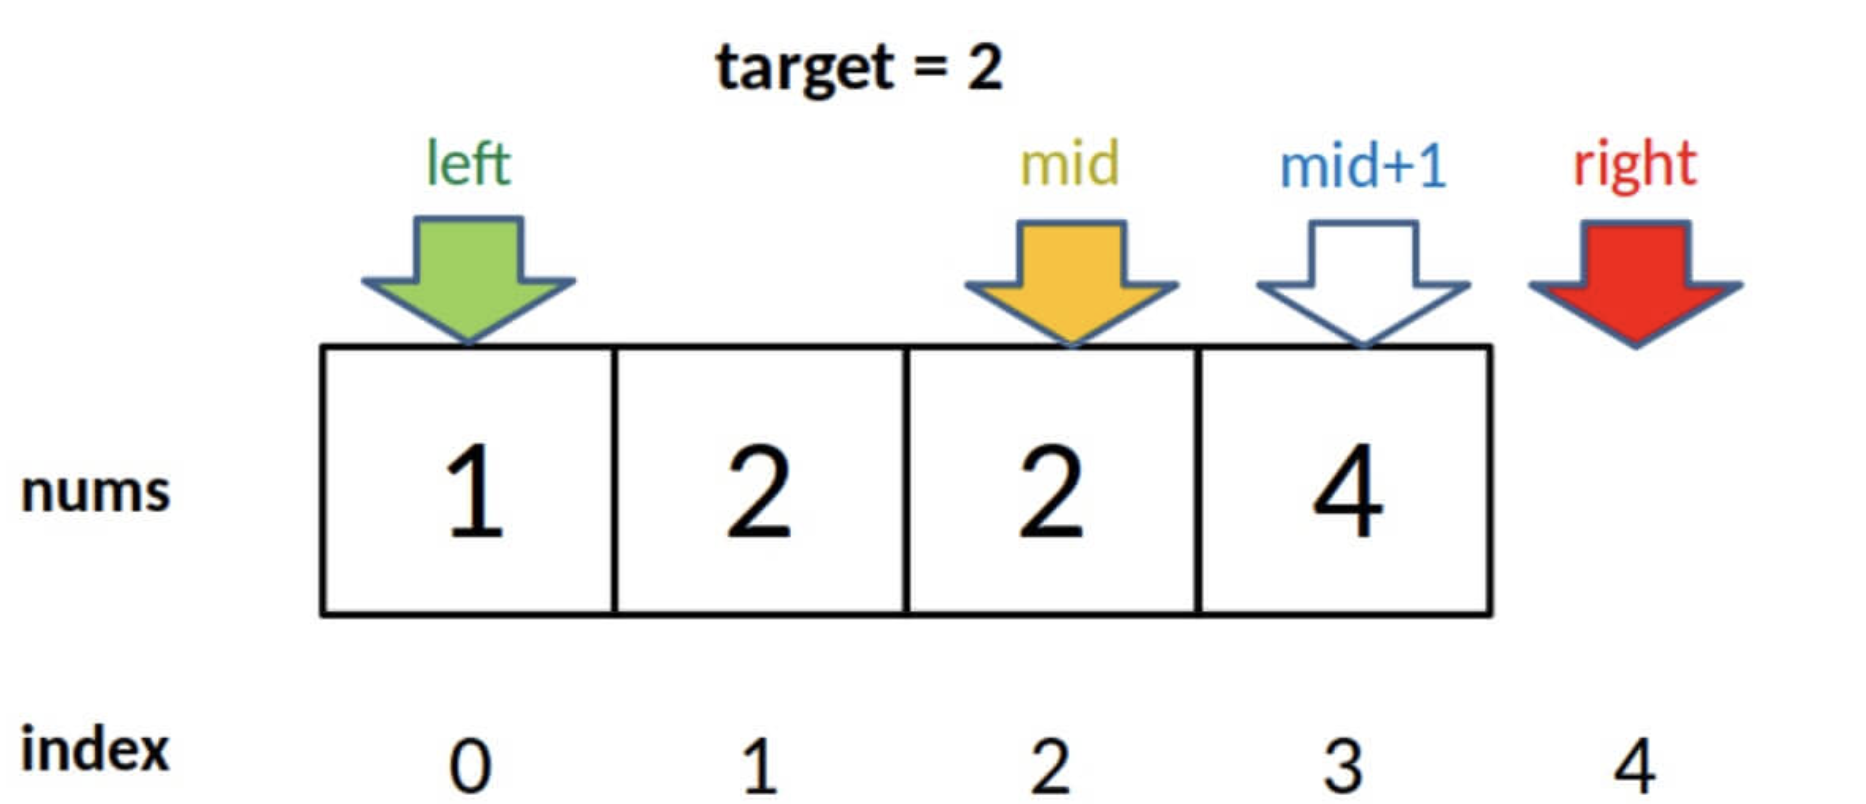
\includegraphics[width=1\textwidth]{fig/Binary_Search_3.png}
\end{figure}
因为我们对 left 的更新必须是 left = mid + 1,就是说 while 循环结束时,nums[left] 一定不等于 target 了,而 nums[left-1] 可能是 target。

至于为什么 left 的更新必须是 left = mid + 1,同左侧边界搜索,就不再赘述。

\subsubsection{为什么没有返回 -1 的操作?}
为什么没有返回 -1 的操作?如果 nums 中不存在 target 这个值,怎么办?

答:类似之前的左侧边界搜索,因为 while 的终止条件是 left == right,就是说 left 的取值范围是 [0, nums.length],所以可以添加两行代码,正确地返回 -1:
\begin{lstlisting}
while (left < right) {
    // ...
}
if (left == 0) return -1;
return nums[left-1] == target ? (left-1) : -1;
\end{lstlisting}

\subsubsection{是否也可以把这个算法的「搜索区间」也统一成两端都闭的形式呢?}
答:当然可以,类似搜索左侧边界的统一写法,其实只要改两个地方就行了:
\begin{lstlisting}
int right_bound(int[] nums, int target) {
    int left = 0, right = nums.length - 1;
    while (left <= right) {
        int mid = left + (right - left) / 2;
        if (nums[mid] < target) {
            left = mid + 1;
        } else if (nums[mid] > target) {
            right = mid - 1;
        } else if (nums[mid] == target) {
            // 这里改成收缩左侧边界即可
            left = mid + 1;
        }
    }
    // 这里改为检查 right 越界的情况,见下图
    if (right < 0 || nums[right] != target)
        return -1;
    return right;
}
\end{lstlisting}

当 target 比所有元素都小时,right 会被减到 -1,所以需要在最后防止越界:
\begin{figure}[H]
    \centering
    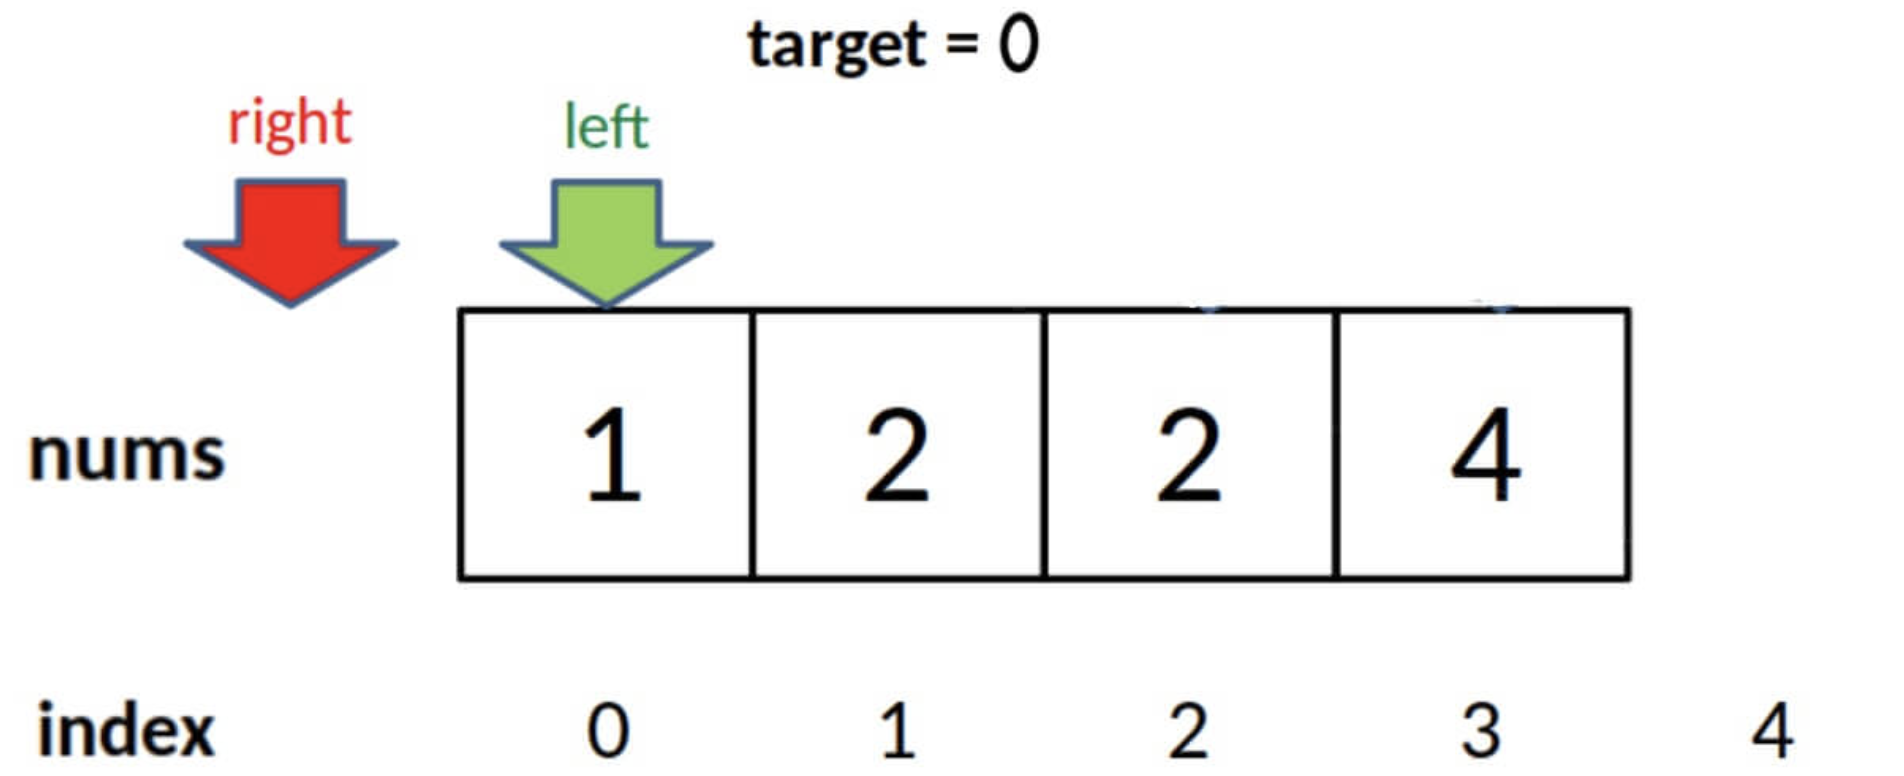
\includegraphics[width=1\textwidth]{fig/Binary_Search_4.png}
\end{figure}

至此,搜索右侧边界的二分查找的两种写法也完成了,其实将「搜索区间」统一成两端都闭反而更容易记忆,你说是吧?

\subsection{逻辑统一}
来梳理一下这些细节差异的因果逻辑:

\subsubsection{最基本的二分查找算法}
\begin{framed}
因为我们初始化 right = nums.length - 1
所以决定了我们的「搜索区间」是 [left, right]
所以决定了 while (left <= right)
同时也决定了 left = mid+1 和 right = mid-1

因为我们只需找到一个 target 的索引即可
所以当 nums[mid] == target 时可以立即返回
\end{framed}

\subsubsection{寻找左侧边界的二分查找}
\begin{framed}
因为我们初始化 right = nums.length
所以决定了我们的「搜索区间」是 [left, right)
所以决定了 while (left < right)
同时也决定了 left = mid + 1 和 right = mid

因为我们需找到 target 的最左侧索引
所以当 nums[mid] == target 时不要立即返回
而要收紧右侧边界以锁定左侧边界
\end{framed}

\subsubsection{寻找右侧边界的二分查找}
\begin{framed}
因为我们初始化 right = nums.length
所以决定了我们的「搜索区间」是 [left, right)
所以决定了 while (left < right)
同时也决定了 left = mid + 1 和 right = mid

因为我们需找到 target 的最右侧索引
所以当 nums[mid] == target 时不要立即返回
而要收紧左侧边界以锁定右侧边界

又因为收紧左侧边界时必须 left = mid + 1
所以最后无论返回 left 还是 right,必须减一
\end{framed}

\subsubsection{统一形式}
对于寻找左右边界的二分搜索,常见的手法是使用左闭右开的「搜索区间」,我们还根据逻辑将「搜索区间」全都统一成了两端都闭,便于记忆,只要修改两处即可变化出三种写法:
\begin{lstlisting}
int binary_search(int[] nums, int target) {
    int left = 0, right = nums.length - 1; 
    while(left <= right) {
        int mid = left + (right - left) / 2;
        if (nums[mid] < target) {
            left = mid + 1;
        } else if (nums[mid] > target) {
            right = mid - 1; 
        } else if(nums[mid] == target) {
            // 直接返回
            return mid;
        }
    }
    // 直接返回
    return -1;
}

int left_bound(int[] nums, int target) {
    int left = 0, right = nums.length - 1;
    while (left <= right) {
        int mid = left + (right - left) / 2;
        if (nums[mid] < target) {
            left = mid + 1;
        } else if (nums[mid] > target) {
            right = mid - 1;
        } else if (nums[mid] == target) {
            // 别返回,锁定左侧边界
            right = mid - 1;
        }
    }
    // 最后要检查 left 越界的情况
    if (left >= nums.length || nums[left] != target)
        return -1;
    return left;
}

int right_bound(int[] nums, int target) {
    int left = 0, right = nums.length - 1;
    while (left <= right) {
        int mid = left + (right - left) / 2;
        if (nums[mid] < target) {
            left = mid + 1;
        } else if (nums[mid] > target) {
            right = mid - 1;
        } else if (nums[mid] == target) {
            // 别返回,锁定右侧边界
            left = mid + 1;
        }
    }
    // 最后要检查 right 越界的情况
    if (right < 0 || nums[right] != target)
        return -1;
    return right;
}
\end{lstlisting}

\section{双指针技巧}
\url{https://github.com/labuladong/fucking-algorithm/blob/master/%E7%AE%97%E6%B3%95%E6%80%9D%E7%BB%B4%E7%B3%BB%E5%88%97/%E5%8F%8C%E6%8C%87%E9%92%88%E6%8A%80%E5%B7%A7.md}

我把双指针技巧再分为两类,一类是「快慢指针」,一类是「左右指针」。前者解决主要解决链表中的问题,比如典型的判定链表中是否包含环;后者主要解决数组(或者字符串)中的问题,比如二分查找。

\subsection{快慢指针的常见算法}
快慢指针一般都初始化指向链表的头结点 head,前进时快指针 fast 在前,慢指针 slow 在后,巧妙解决一些链表中的问题。

\subsubsection{判定链表中是否含有环}
单链表的特点是每个节点只知道下一个节点,所以一个指针的话无法判断链表中是否含有环的。

如果链表中不含环,那么这个指针最终会遇到空指针 null 表示链表到头了,这还好说,可以判断该链表不含环。
\begin{lstlisting}
boolean hasCycle(ListNode head) {
    while (head != null)
        head = head.next;
    return false;
}
\end{lstlisting}

但是如果链表中含有环,那么这个指针就会陷入死循环,因为环形数组中没有 null 指针作为尾部节点。

经典解法就是用两个指针,一个跑得快,一个跑得慢。如果不含有环,跑得快的那个指针最终会遇到 null,说明链表不含环;如果含有环,快指针最终会超慢指针一圈,和慢指针相遇,说明链表含有环。
\begin{lstlisting}
boolean hasCycle(ListNode head) {
    ListNode fast, slow;
    fast = slow = head;
    while (fast != null && fast.next != null) {
        fast = fast.next.next;
        slow = slow.next;
        
        if (fast == slow) return true;
    }
    return false;
}
\end{lstlisting}

\subsubsection{已知链表中含有环,返回这个环的起始位置}
\begin{figure}[H]
    \centering
    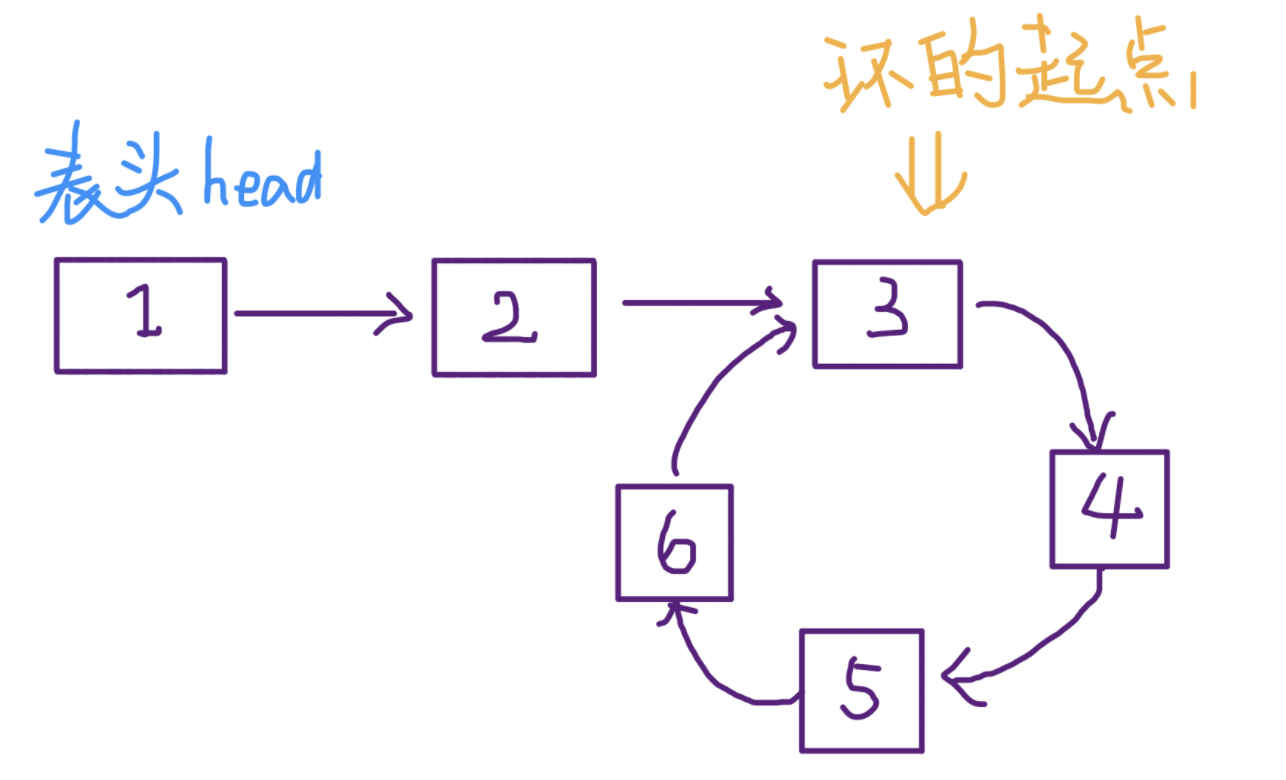
\includegraphics[width=.6\textwidth]{fig/Double_Pointers_1.png}
\end{figure}

这个问题一点都不困难,有点类似脑筋急转弯,先直接看代码:
\begin{lstlisting}
ListNode detectCycle(ListNode head) {
    ListNode fast, slow;
    fast = slow = head;
    while (fast != null && fast.next != null) {
        fast = fast.next.next;
        slow = slow.next;
        if (fast == slow) break;
    }
    // 上面的代码类似 hasCycle 函数
    slow = head;
    while (slow != fast) {
        fast = fast.next;
        slow = slow.next;
    }
    return slow;
}
\end{lstlisting}

可以看到,当快慢指针相遇时,让其中任一个指针指向头节点,然后让它俩以相同速度前进,再次相遇时所在的节点位置就是环开始的位置。这是为什么呢?

第一次相遇时,假设慢指针 slow 走了 k 步,那么快指针 fast 一定走了 2k 步,也就是说比 slow 多走了 k 步(环长度的倍数)。
\begin{figure}[H]
    \centering
    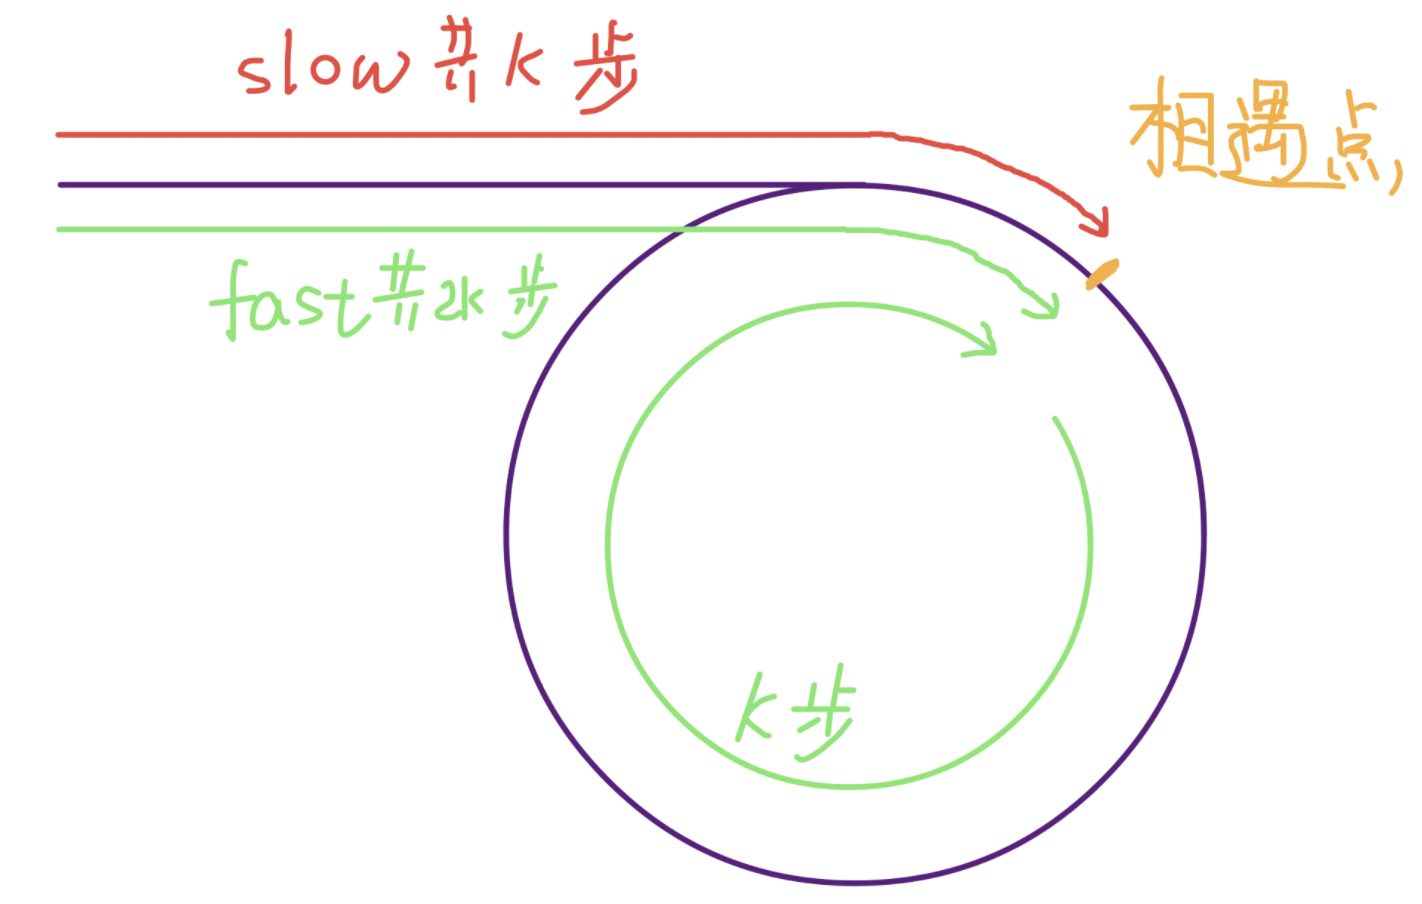
\includegraphics[width=.6\textwidth]{fig/Double_Pointers_2.png}
\end{figure}

设相遇点距环的起点的距离为 m,那么环的起点距头结点 head 的距离为 k - m,也就是说如果从 head 前进 k - m 步就能到达环起点。

巧的是,如果从相遇点继续前进 k - m 步,也恰好到达环起点。
\begin{figure}[H]
    \centering
    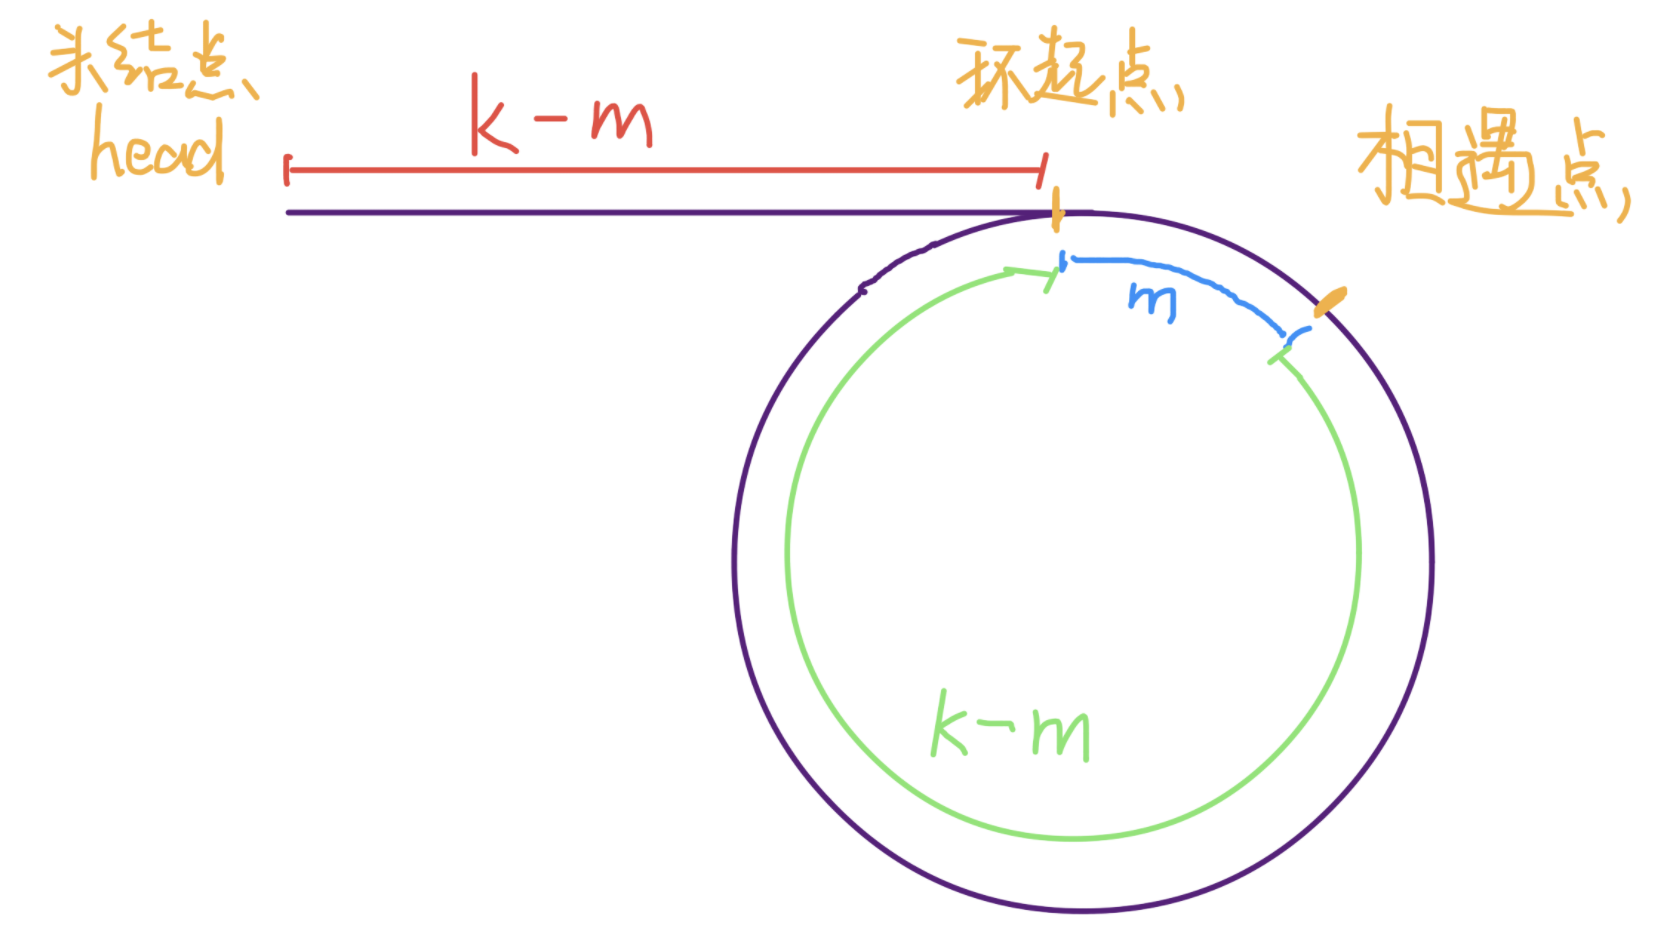
\includegraphics[width=.6\textwidth]{fig/Double_Pointers_3.png}
\end{figure}

所以,只要我们把快慢指针中的任一个重新指向 head,然后两个指针同速前进,k - m 步后就会相遇,相遇之处就是环的起点了。

\subsubsection{寻找链表的中点}
类似上面的思路,我们还可以让快指针一次前进两步,慢指针一次前进一步,当快指针到达链表尽头时,慢指针就处于链表的中间位置。
\begin{lstlisting}
while (fast != null && fast.next != null) {
    fast = fast.next.next;
    slow = slow.next;
}
// slow 就在中间位置
return slow;
\end{lstlisting}

当链表的长度是奇数时,slow 恰巧停在中点位置;如果长度是偶数,slow 最终的位置是中间偏右:
\begin{figure}[H]
    \centering
    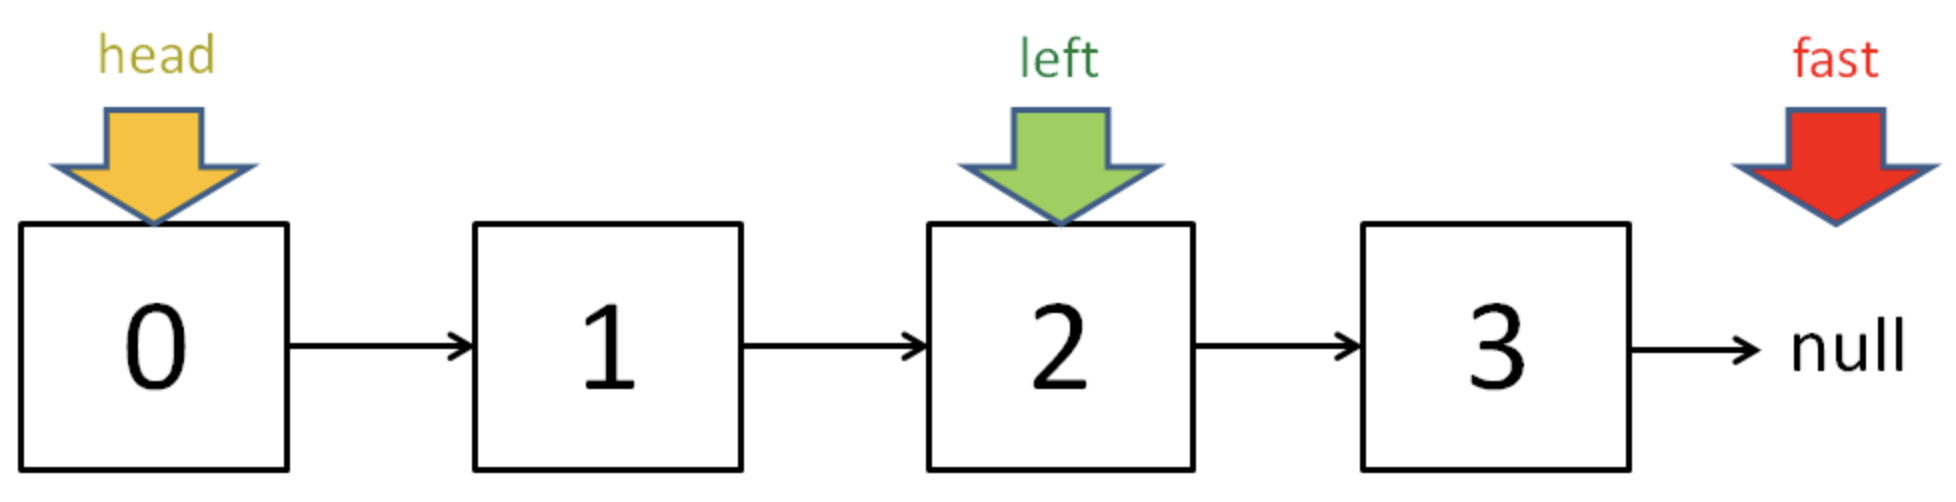
\includegraphics[width=.6\textwidth]{fig/Double_Pointers_4.png}
\end{figure}
	
\textbf{寻找链表中点的一个重要作用是对链表进行归并排序}。

回想数组的归并排序:求中点索引递归地把数组二分,最后合并两个有序数组。对于链表,合并两个有序链表是很简单的,难点就在于二分。

但是现在你学会了找到链表的中点,就能实现链表的二分了。关于归并排序的具体内容本文就不具体展开了。

\subsubsection{寻找链表的倒数第 k 个元素}
我们的思路还是使用快慢指针,让快指针先走 k 步,然后快慢指针开始同速前进。这样当快指针走到链表末尾 null 时,慢指针所在的位置就是倒数第 k 个链表节点(为了简化,假设 k 不会超过链表长度):
\begin{lstlisting}
ListNode slow, fast;
slow = fast = head;
while (k-- > 0) 
    fast = fast.next;

while (fast != null) {
    slow = slow.next;
    fast = fast.next;
}
return slow;
\end{lstlisting}

\subsection{左右指针的常用算法}
左右指针在数组中实际是指两个索引值,一般初始化为 left = 0, right = nums.length - 1 。

\subsubsection{二分查找}
前文「二分查找」有详细讲解,这里只写最简单的二分算法,旨在突出它的双指针特性:
\begin{lstlisting}
int binarySearch(int[] nums, int target) {
    int left = 0; 
    int right = nums.length - 1;
    while(left <= right) {
        int mid = (right + left) / 2;
        if(nums[mid] == target)
            return mid; 
        else if (nums[mid] < target)
            left = mid + 1; 
        else if (nums[mid] > target)
            right = mid - 1;
    }
    return -1;
}
\end{lstlisting}

\subsubsection{两数之和}
\begin{figure}[H]
    \centering
    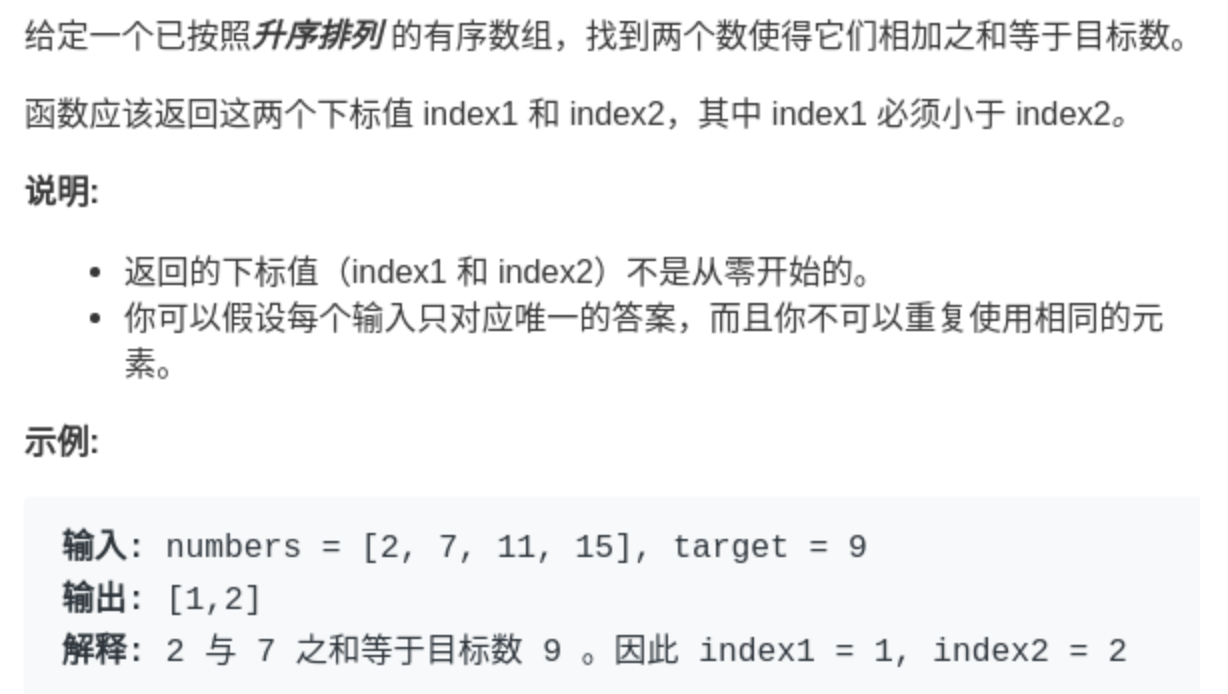
\includegraphics[width=.6\textwidth]{fig/Double_Pointers_5.png}
\end{figure}

只要数组有序,就应该想到双指针技巧。这道题的解法有点类似二分查找,通过调节 left 和 right 可以调整 sum 的大小:
\begin{lstlisting}
int[] twoSum(int[] nums, int target) {
    int left = 0, right = nums.length - 1;
    while (left < right) {
        int sum = nums[left] + nums[right];
        if (sum == target) {
            // 题目要求的索引是从 1 开始的
            return new int[]{left + 1, right + 1};
        } else if (sum < target) {
            left++; // 让 sum 大一点
        } else if (sum > target) {
            right--; // 让 sum 小一点
        }
    }
    return new int[]{-1, -1};
}
\end{lstlisting}

\subsubsection{反转数组}
\begin{lstlisting}
void reverse(int[] nums) {
    int left = 0;
    int right = nums.length - 1;
    while (left < right) {
        // swap(nums[left], nums[right])
        int temp = nums[left];
        nums[left] = nums[right];
        nums[right] = temp;
        left++; right--;
    }
}
\end{lstlisting}

\subsubsection{滑动窗口算法}
这也许是双指针技巧的最高境界了,如果掌握了此算法,可以解决一大类子字符串匹配的问题,不过「滑动窗口」稍微比上述的这些算法复杂些。

见下文。

\section{滑动窗口}
\url{https://github.com/labuladong/fucking-algorithm/blob/master/%E7%AE%97%E6%B3%95%E6%80%9D%E7%BB%B4%E7%B3%BB%E5%88%97/%E6%BB%91%E5%8A%A8%E7%AA%97%E5%8F%A3%E6%8A%80%E5%B7%A7.md}

\subsection{最小覆盖子串}
\begin{figure}[H]
    \centering
    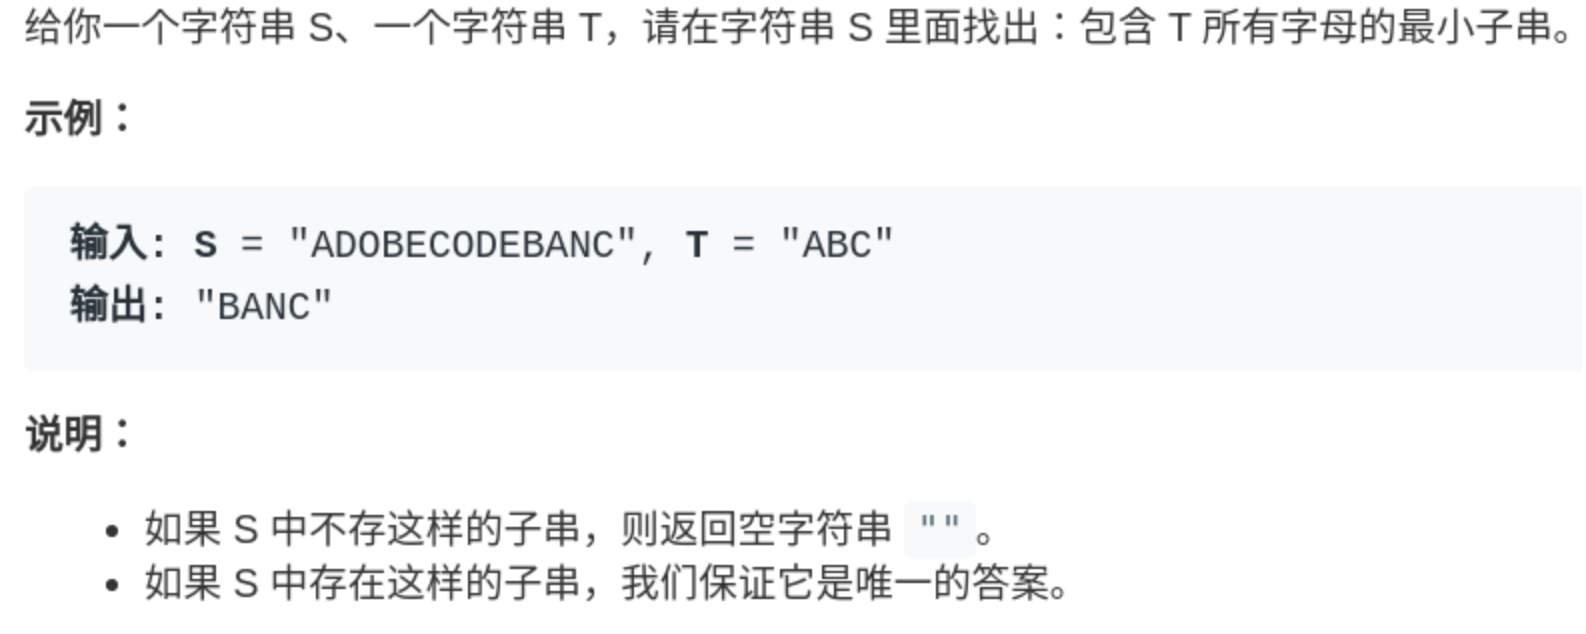
\includegraphics[width=.8\textwidth]{fig/Sliding_Window_1.png}
\end{figure}
题目不难理解,就是说要在 S(source) 中找到包含 T(target) 中全部字母的一个子串,顺序无所谓,但这个子串一定是所有可能子串中最短的。

如果我们使用暴力解法,代码大概是这样的:
\begin{lstlisting}
for (int i = 0; i < s.size(); i++)
    for (int j = i + 1; j < s.size(); j++)
        if s[i:j] 包含 t 的所有字母:
            更新答案
\end{lstlisting}

思路很直接吧,但是显然,这个算法的复杂度肯定大于$ O(N^2)$了,不好。

滑动窗口算法的思路是这样:
\begin{itemize}
\setlength{\itemsep}{0pt}
\setlength{\parsep}{0pt}
\setlength{\parskip}{0pt}
    \item 我们在字符串 S 中使用双指针中的左右指针技巧,初始化 left = right = 0,把索引闭区间 [left, right] 称为一个「窗口」;
    \item 我们先不断地增加 right 指针扩大窗口 [left, right],直到窗口中的字符串符合要求(包含了 T 中的所有字符);
    \item 此时,我们停止增加 right,转而不断增加 left 指针缩小窗口 [left, right],直到窗口中的字符串不再符合要求(不包含 T 中的所有字符了)。同时,每次增加 left,我们都要更新一轮结果;
    \item 重复第 2 和第 3 步,直到 right 到达字符串 S 的尽头。
\end{itemize}

这个思路其实也不难,\textbf{第 2 步相当于在寻找一个「可行解」,然后第 3 步在优化这个「可行解」,最终找到最优解}。左右指针轮流前进,窗口大小增增减减,窗口不断向右滑动。

下面画图理解一下,needs 和 window 相当于计数器,分别记录 T 中字符出现次数和窗口中的相应字符的出现次数。

初始状态:
\begin{figure}[H]
    \centering
    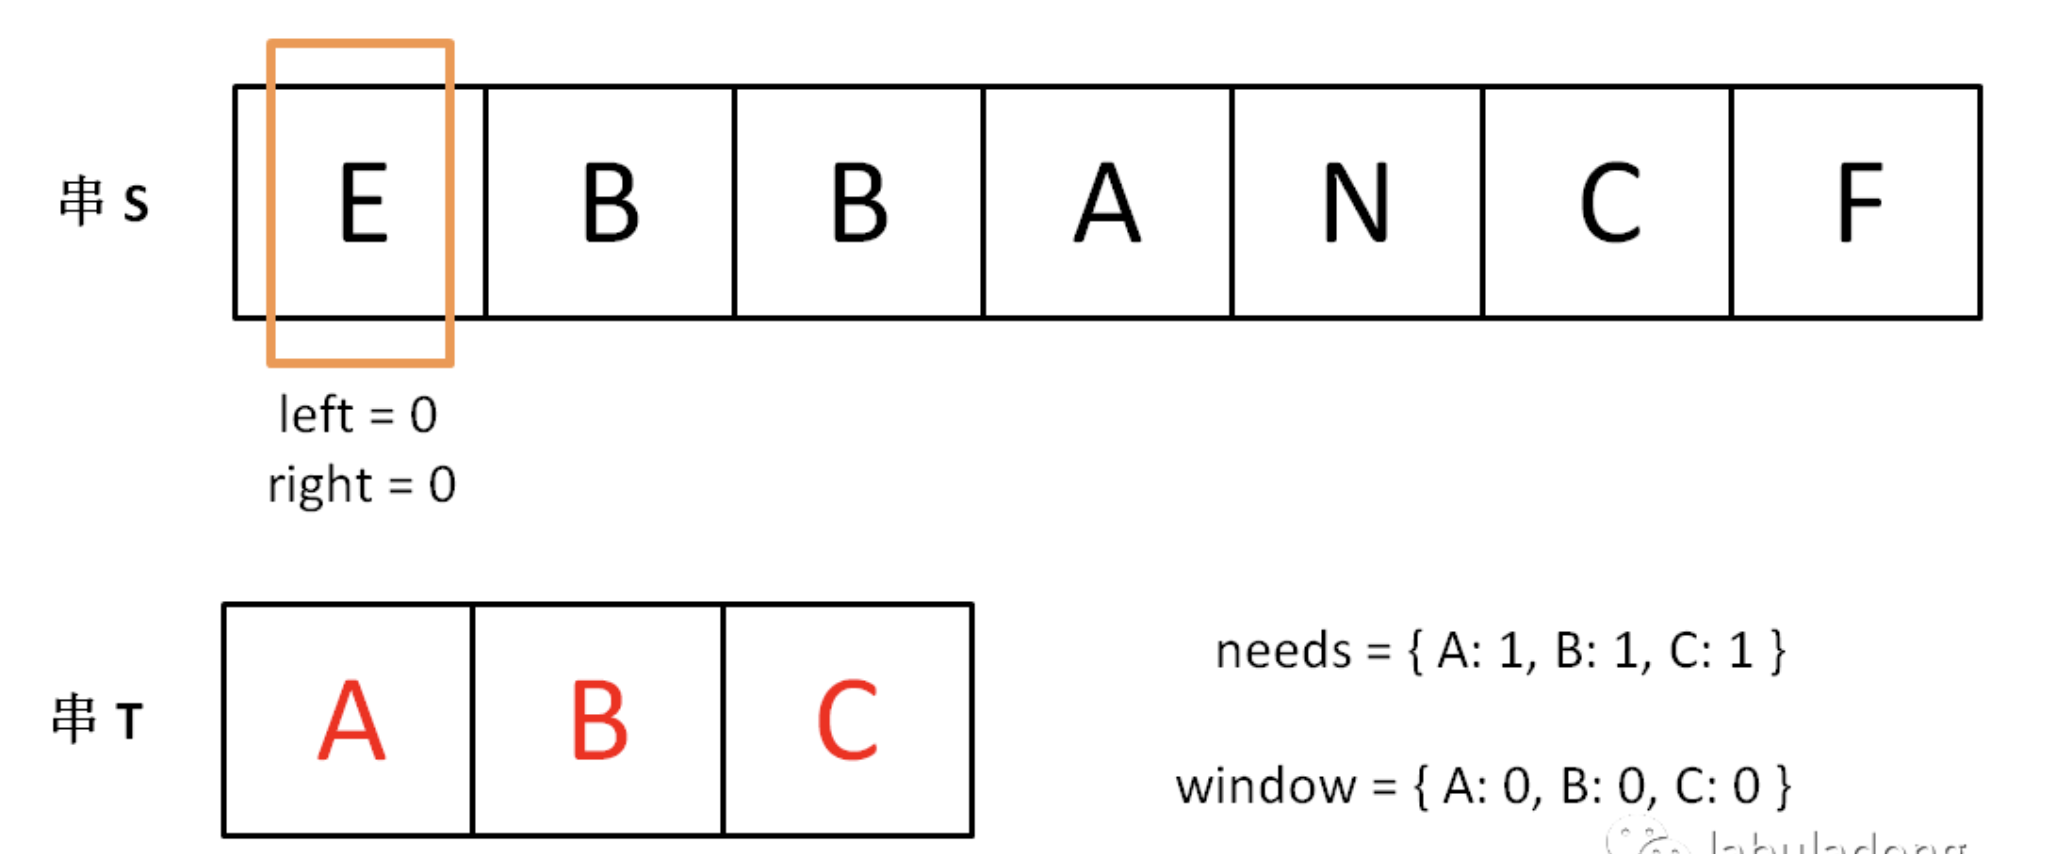
\includegraphics[width=.6\textwidth]{fig/Sliding_Window_2.png}
\end{figure}

增加 right,直到窗口 [left, right] 包含了 T 中所有字符:
\begin{figure}[H]
    \centering
    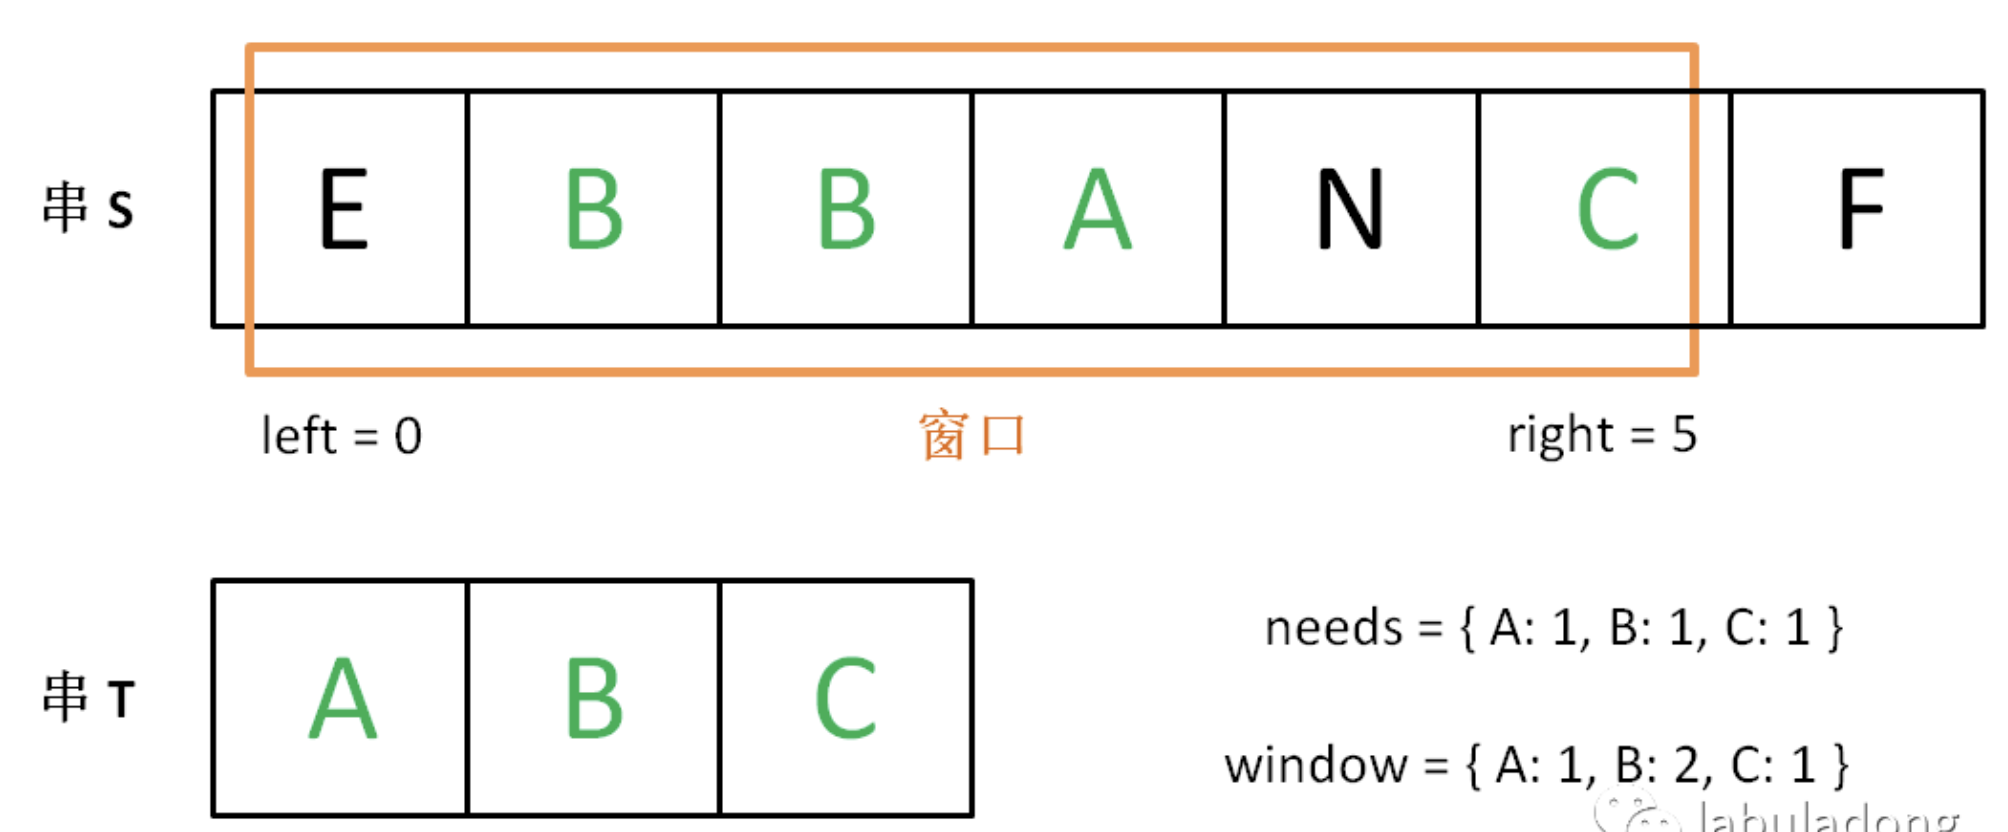
\includegraphics[width=.6\textwidth]{fig/Sliding_Window_3.png}
\end{figure}

现在开始增加 left,缩小窗口 [left, right]。
\begin{figure}[H]
    \centering
    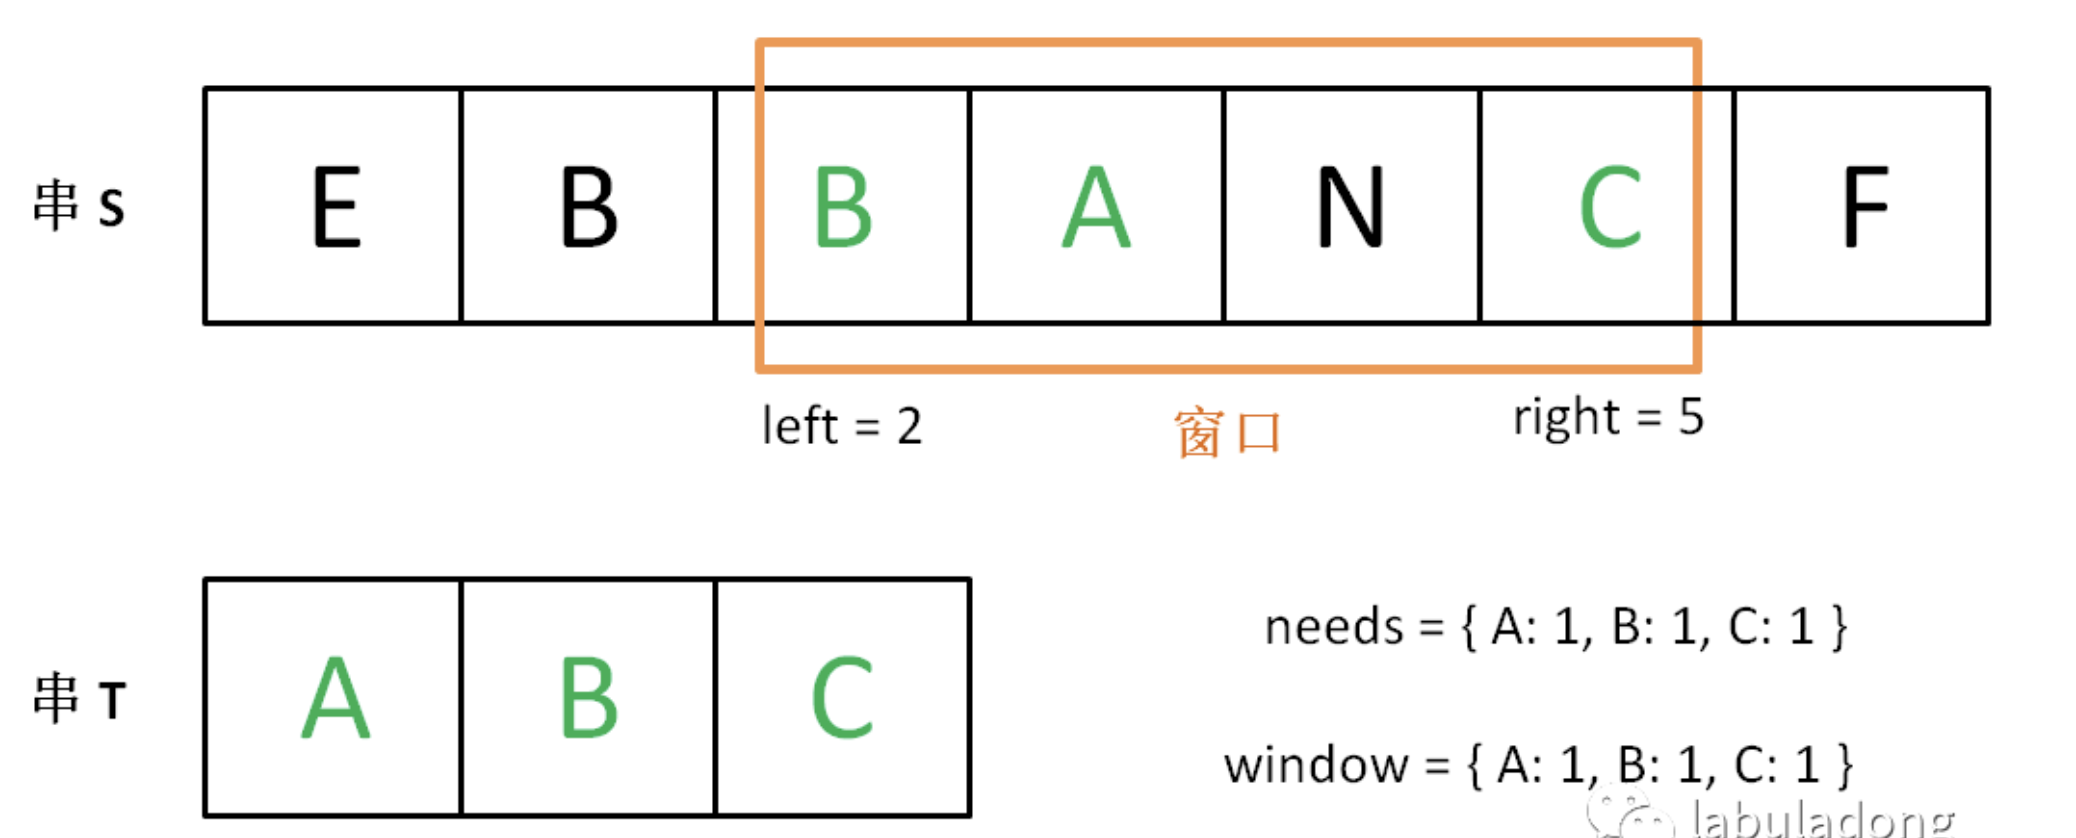
\includegraphics[width=.6\textwidth]{fig/Sliding_Window_4.png}
\end{figure}

直到窗口中的字符串不再符合要求,left 不再继续移动。
\begin{figure}[H]
    \centering
    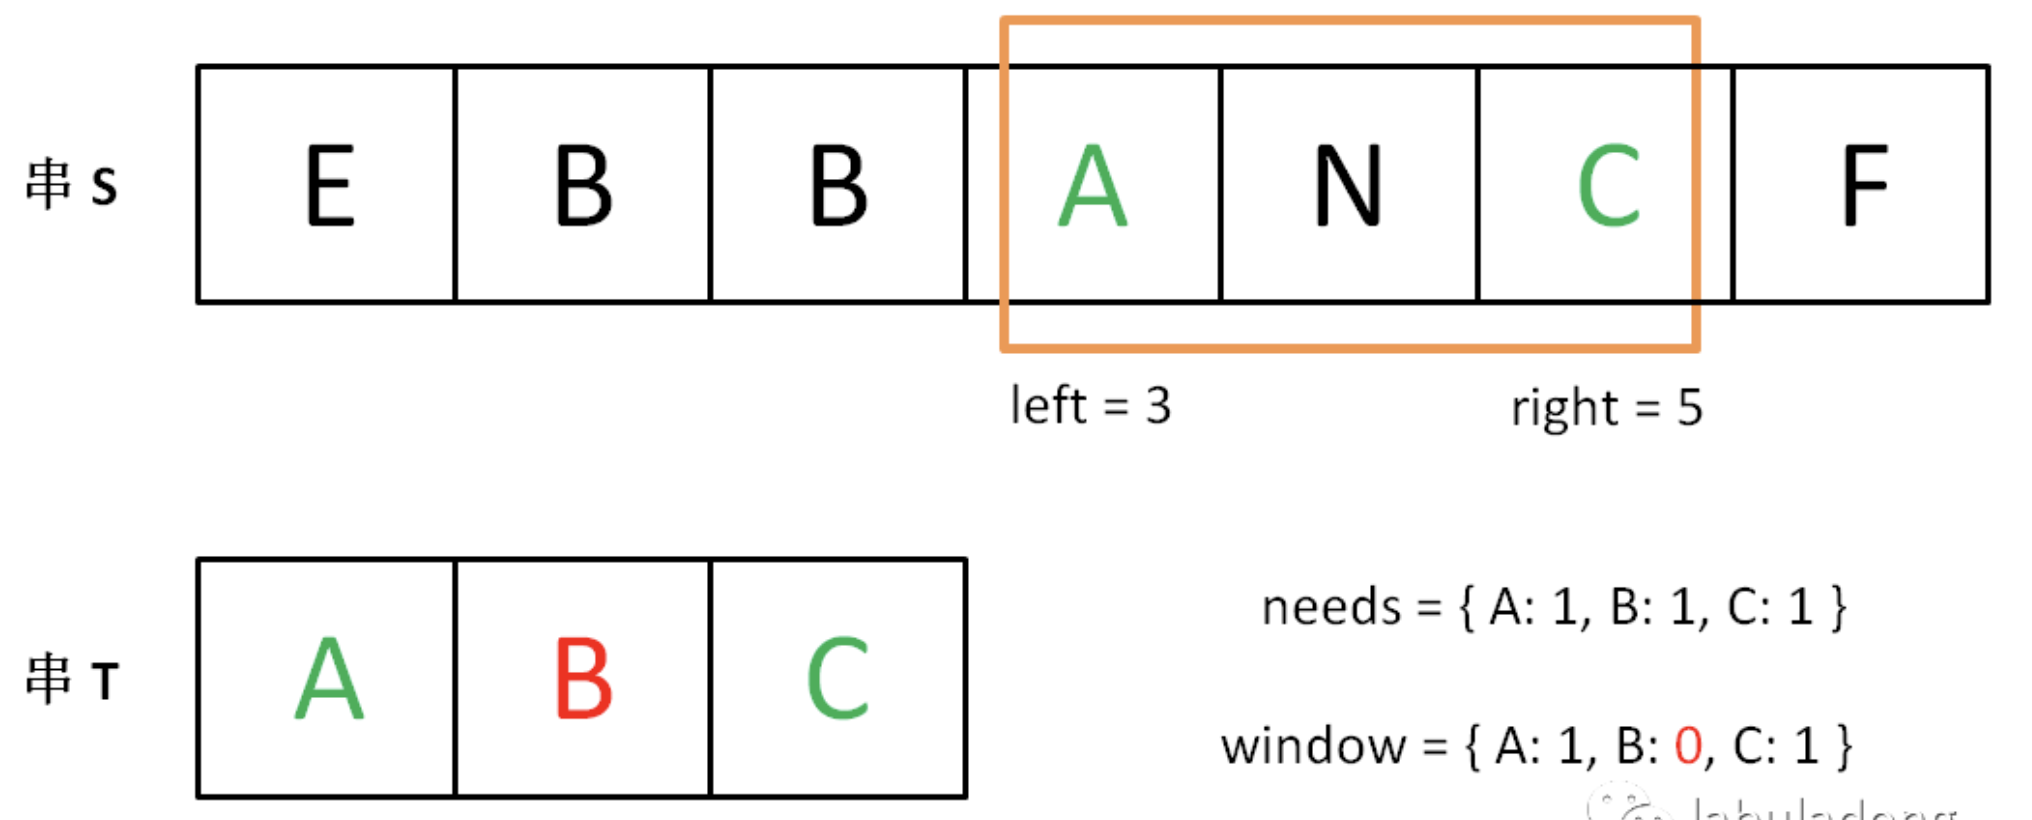
\includegraphics[width=.6\textwidth]{fig/Sliding_Window_5.png}
\end{figure}

之后重复上述过程,先移动 right,再移动 left…… 直到 right 指针到达字符串 S 的末端,算法结束。

如果你能够理解上述过程,恭喜,你已经完全掌握了滑动窗口算法思想。至于如何具体到问题,如何得出此题的答案,都是编程问题,等会提供一套模板,理解一下就会了。

上述过程可以简单地写出如下伪码框架:
\begin{lstlisting}
string s, t;
// 在 s 中寻找 t 的「最小覆盖子串」
int left = 0, right = 0;
string res = s;

while(right < s.size()) {
    window.add(s[right]);
    right++;
    // 如果符合要求,移动 left 缩小窗口
    while (window 符合要求) {
        // 如果这个窗口的子串更短,则更新 res
        res = minLen(res, window);
        window.remove(s[left]);
        left++;
    }
}
return res;
\end{lstlisting}

如果上述代码你也能够理解,那么你离解题更近了一步。现在就剩下一个比较棘手的问题:如何判断 window 即子串 s[left...right] 是否符合要求,是否包含 t 的所有字符呢?

可以用两个哈希表当作计数器解决。用一个哈希表 needs 记录字符串 t 中包含的字符及出现次数,用另一个哈希表 window 记录当前「窗口」中包含的字符及出现的次数,如果 window 包含所有 needs 中的键,且这些键对应的值都大于等于 needs 中的值,那么就可以知道当前「窗口」符合要求了,可以开始移动 left 指针了。

现在将上面的框架继续细化:
\begin{lstlisting}
string s, t;
// 在 s 中寻找 t 的「最小覆盖子串」
int left = 0, right = 0;
string res = s;

// 相当于两个计数器
unordered_map<char, int> window;
unordered_map<char, int> needs;
for (char c : t) needs[c]++;

// 记录 window 中已经有多少字符符合要求了
int match = 0; 

while (right < s.size()) {
    char c1 = s[right];
    if (needs.count(c1)) {
        window[c1]++; // 加入 window
        if (window[c1] == needs[c1])
            // 字符 c1 的出现次数符合要求了
            match++;
    }
    right++;

    // window 中的字符串已符合 needs 的要求了
    while (match == needs.size()) {
        // 更新结果 res
        res = minLen(res, window);
        char c2 = s[left];
        if (needs.count(c2)) {
            window[c2]--; // 移出 window
            if (window[c2] < needs[c2])
                // 字符 c2 出现次数不再符合要求
                match--;
        }
        left++;
    }
}
return res;
\end{lstlisting}

上述代码已经具备完整的逻辑了,只有一处伪码,即更新 res 的地方,不过这个问题太好解决了,直接看解法吧!
\begin{lstlisting}
string minWindow(string s, string t) {
    // 记录最短子串的开始位置和长度
    int start = 0, minLen = INT_MAX;
    int left = 0, right = 0;
    
    unordered_map<char, int> window;
    unordered_map<char, int> needs;
    for (char c : t) needs[c]++;
    
    int match = 0;
    
    while (right < s.size()) {
        char c1 = s[right];
        if (needs.count(c1)) {
            window[c1]++;
            if (window[c1] == needs[c1]) 
                match++;
        }
        right++;
        
        while (match == needs.size()) {
            if (right - left < minLen) {
                // 更新最小子串的位置和长度
                start = left;
                minLen = right - left;
            }
            char c2 = s[left];
            if (needs.count(c2)) {
                window[c2]--;
                if (window[c2] < needs[c2])
                    match--;
            }
            left++;
        }
    }
    return minLen == INT_MAX ? "" : s.substr(start, minLen);
}
\end{lstlisting}

这个算法的时间复杂度是 $O(M + N)$,M 和 N 分别是字符串 S 和 T 的长度。因为我们先用 for 循环遍历了字符串 T 来初始化 needs,时间 O(N),之后的两个 while 循环最多执行 2M 次,时间 O(M)。

读者也许认为嵌套的 while 循环复杂度应该是平方级,但是你这样想,while 执行的次数就是双指针 left 和 right 走的总路程,最多是 2M 嘛。

\subsection{找到字符串中所有字母异位词}
\begin{figure}[H]
    \centering
    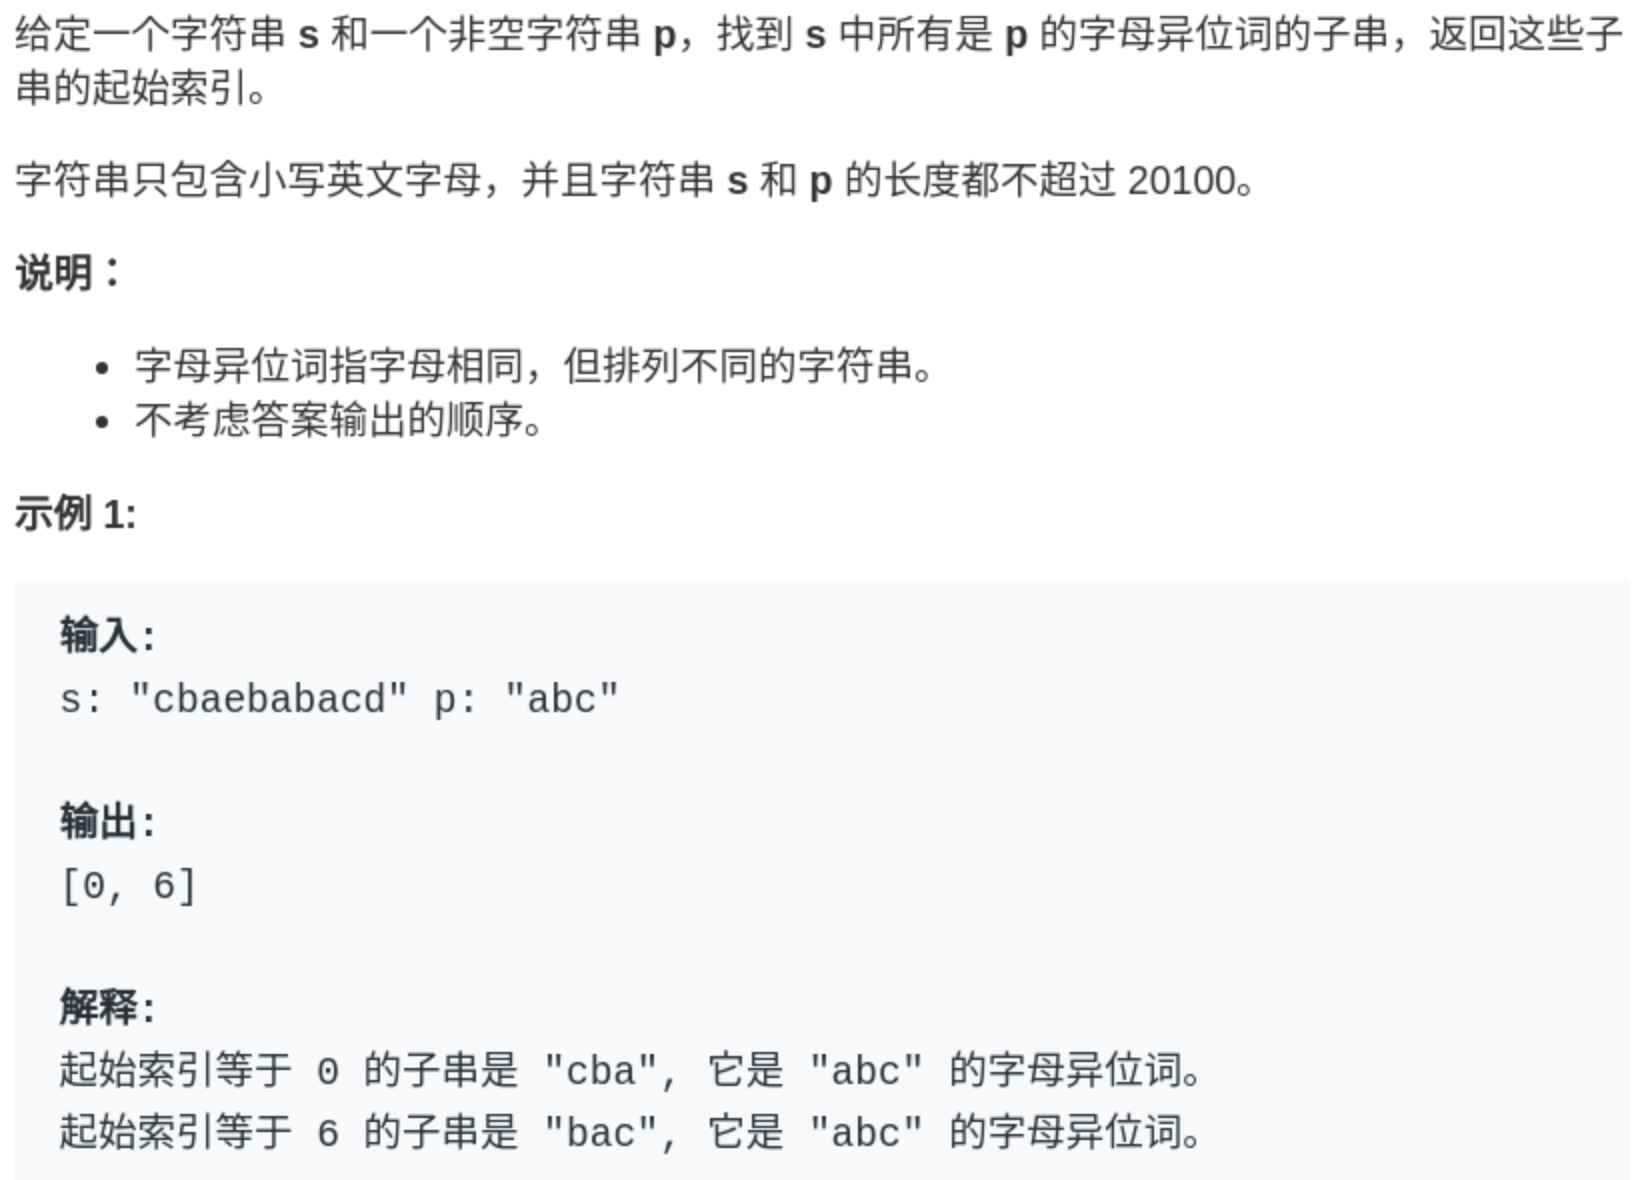
\includegraphics[width=.8\textwidth]{fig/Sliding_Window_6.png}
\end{figure}

这道题的难度是 Easy,这个 Easy 是属于了解双指针技巧的人的,只要把上一道题的代码改中更新 res 部分的代码稍加修改就成了这道题的解:
\begin{lstlisting}
vector<int> findAnagrams(string s, string t) {
    // 用数组记录答案
    vector<int> res;
    int left = 0, right = 0;
    unordered_map<char, int> needs;
    unordered_map<char, int> window;
    for (char c : t) needs[c]++;
    int match = 0;
    
    while (right < s.size()) {
        char c1 = s[right];
        if (needs.count(c1)) {
            window[c1]++;
            if (window[c1] == needs[c1])
                match++;
        }
        right++;

        while (match == needs.size()) {
            // 如果 window 的大小合适
            // 就把起始索引 left 加入结果
            if (right - left == t.size()) {
                res.push_back(left);
            }
            char c2 = s[left];
            if (needs.count(c2)) {
                window[c2]--;
                if (window[c2] < needs[c2])
                    match--;
            }
            left++;
        }
    }
    return res;
}
\end{lstlisting}

因为这道题和上一道的场景类似,也需要 window 中包含串 t 的所有字符,但上一道题要找长度最短的子串,这道题要找长度相同的子串,也就是「字母异位词」嘛。

\subsection{无重复字符的最长子串}
\begin{figure}[H]
    \centering
    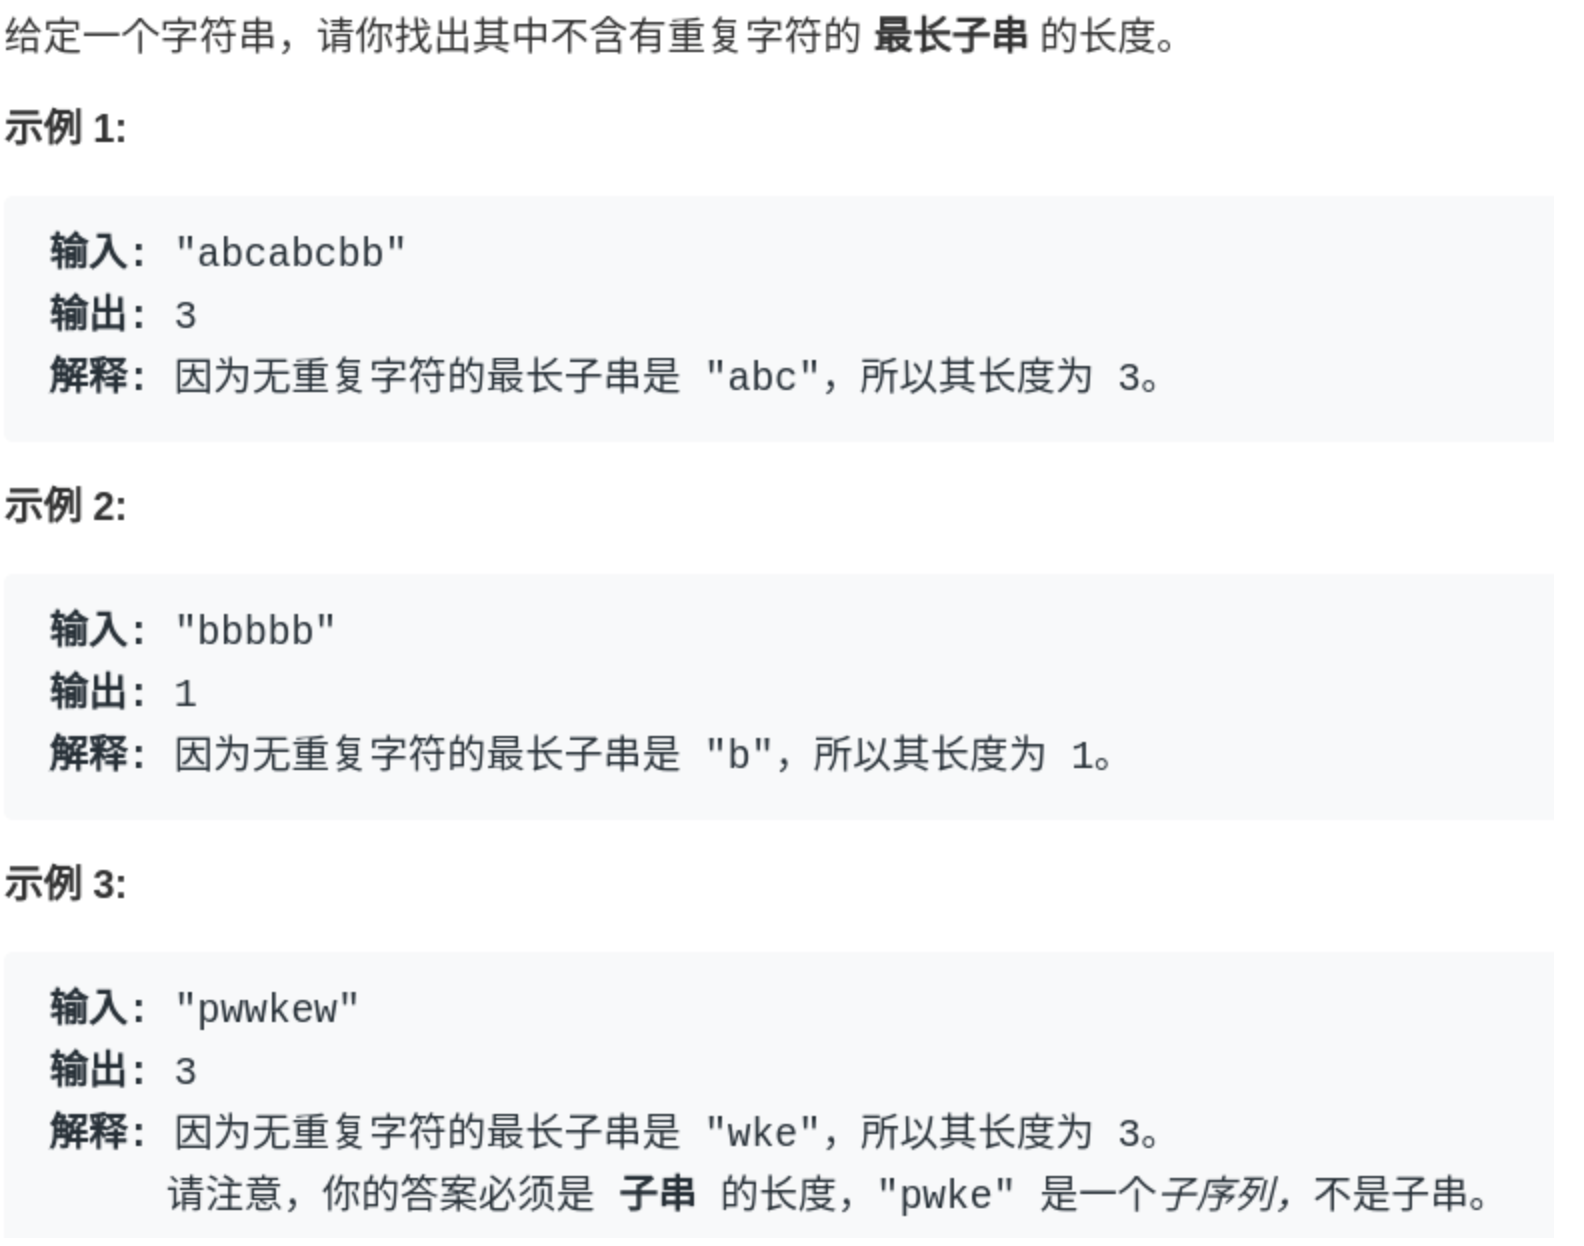
\includegraphics[width=.8\textwidth]{fig/Sliding_Window_7.png}
\end{figure}

遇到子串问题,首先想到的就是滑动窗口技巧。

类似之前的思路,使用 window 作为计数器记录窗口中的字符出现次数,然后先向右移动 right,当 window 中出现重复字符时,开始移动 left 缩小窗口,如此往复:
\begin{lstlisting}
int lengthOfLongestSubstring(string s) {
    int left = 0, right = 0;
    unordered_map<char, int> window;
    int res = 0; // 记录最长长度

    while (right < s.size()) {
        char c1 = s[right];
        window[c1]++;
        right++;
        // 如果 window 中出现重复字符
        // 开始移动 left 缩小窗口
        while (window[c1] > 1) {
            char c2 = s[left];
            window[c2]--;
            left++;
        }
        res = max(res, right - left);
    }
    return res;
}
\end{lstlisting}
需要注意的是,因为我们要求的是最长子串,所以需要在每次移动 right 增大窗口时更新 res,而不是像之前的题目在移动 left 缩小窗口时更新 res。

\subsection{总结}
通过上面三道题,我们可以总结出滑动窗口算法的抽象思想:
\begin{lstlisting}
int left = 0, right = 0;

while (right < s.size()) {
    window.add(s[right]);
    right++;
    
    while (valid) {
        window.remove(s[left]);
        left++;
    }
}
\end{lstlisting}

其中 window 的数据类型可以视具体情况而定,比如上述题目都使用哈希表充当计数器,当然你也可以用一个数组实现同样效果,因为我们只处理英文字母。

稍微麻烦的地方就是这个 valid 条件,为了实现这个条件的实时更新,我们可能会写很多代码。比如前两道题,看起来解法篇幅那么长,实际上思想还是很简单,只是大多数代码都在处理这个问题而已。





%\printbibliography
\bibliography{../ref}
\bibliographystyle{IEEEtran}
\end{document}